\documentclass[oneside, eng]{mgr}

\usepackage{polski}
\usepackage[utf8]{inputenc}
\usepackage{amsmath}	
\usepackage{graphicx}
\graphicspath{ {./} }
\usepackage{amsfonts}
\usepackage{hyperref}
\usepackage{tabstackengine}
\usepackage{caption}
\usepackage{subfig}
\usepackage{listings}

\newcommand{\bb}{\textbf}



\title{Biometryczny system kontroli dostępu - przetwarzanie obrazów i przygotowanie danych dla sieci neuronowych}
\engtitle{Biometric access control system - image and data preprocessing for neural nets}
\author{Jędrzej Kozal}
\supervisor{dr  inż. Piotr Ciskowski}

\field{Automatyka i Robotyka (AIR)}
\specialisation{Technologie informacyjne \\ w systemach automatyki (ART)}

\begin{document}
\bibliographystyle{plabbrv}

\maketitle

\linespread{1.5}

\chapter{Wstęp}
Celem pracy jest porównanie metod i algorytmów umożliwiających wykrycie twarzy na zdjęciu oraz wyznaczenie wektora uczącego dla sieci neuronowej na podstawie wykrytego obszaru zdjęcia zawierajacego twarz. Projekt ten jest częścią systemu biometrycznej kontroli dostępu. Za implementację sieci neuronowych oraz analizę algorytmów związanych z sieciami odpowiadał Filip Guzy. Za architekturę systemu oraz komunikację pomiędzy komponentami odpowiadał Michał Leś. 

Celem całego projektu było skonstruowanie prostego systemu kontroli dostępu opartego na rozpoznawaniu twarzy. System ma określać, czy na wykonanym zdjęciu występuje twarz. Po wykryciu twarzy następuje ekstrakcja cech - wyznaczenie wektora cech i przygotowanie wektora uczącego dla sieci. Zadaniem sieci neuronowej jest klasyfikacja użytkownika i podjęcie decyzji czy danemu użytkownikowi powinien zostać przyznany dostęp, czy też nie.

System oryginalnie został zaprojektowany na mikrokomputer Raspberry Pi. W projekcie wykorzystano Raspberry Pi 3. Przy projektowaniu systemu fakt ten miał niebagatelne znaczenie ze względu na ograniczone pokłady mocy obliczeniowej. Architekutra systemu została zaprojektowana w taki sposób, aby system można było z łatwością przenosić na inne platformy. 


\section{Omówienie zagadnienia}

Biometria to nauka zajmująca się mierzeniem cech osobniczych. Jest wykorzystywana w~systemach kontroli dostępu w celu zwiększenia niezawodności i bezpieczeństwa. Użytkownik systemu korzystającego z takiego systemu nie musi pamiętać haseł, nosić przy sobie kart identyfikacyjnych, czy kluczy. Cechy osobnicze dzielmy na fizyczne i behawioralne. Najczęściej przedstawianymi cechami są:

\begin{enumerate}

\item Cechy fizyczne:
	\begin{itemize}
		\item Siatkówka
		\item Tęczówka
		\item Odcisk palca
		\item Twarz
		\item Geometria dłoni
	\end{itemize}

\item Cechy behawioralne:
	\begin{itemize}
		\item Głos
		\item Podpis
		\item Sposób chodzenia
	\end{itemize}

\end{enumerate} 

Cechy najczęściej są unikatowe dla poszczególnych osobników, co zapewnia ich wiarygodność. Biometria cieszy się rosnącą popularnością, ze względu na wiele możliwych zastosowań. Dodatkowo wzrost możliwości obliczeniowych oraz rozwój technik Machine Learning i Pattern Recognition przyczyniają się do znaczących postępów w tej dziedzinie. Metody statystyczne umozliwiają ilościową analizę pomiarów wybranych cech osobniczych. Zastosowanie tanich czujników w urządzeniach produkcji masowej powoduje przenikanie tej dziedziny do życia codziennego. Niektóre smartfony zawierają biometryczne systemy kontroli dostępu. 

Przetworzenie zebranych pomiarów i ich ilościowa analiza, umożliwiająca identyfikację osobnika jest trudnym zadaniem. Wymaga przeniesienia fizycznych pomiarów na bardziej abstrakcyjne poziomy i znalezienie ukrytych zależności. Często bardzo pomocna jest inna reprezentacja danych. 

W realizowanym systemie zdecydowano się na analizowanie twarzy ze względu na łatwą akwizycję cech osobniczych. Przyjęto następujące kroki przetwarzania danych:

\begin{enumerate}

\item Akwizycja obrazu
	
Jako czujnik wykorzystano kamerę mikrokomputera Raspberry Pi. Zawiera ona matrycę OV5647 i umożliwia wykonywanie zdjęć w rozdzielczości 5 MPx. Komunikacja z mikrokomputerem odbywa się przez port CSI. Jest to wygodne rozwiązanie i daje wiele możliwości rozwoju projektu. 
	
\item Przetwarzanie obrazu

Przed operacją wykrywania twarzy z wykorzystaniem kaskad Haara, obraz jest konwertowany do skali szarości. W przypadku ekstrakcji głębi na podstawie obrazów, z~dwóch kamer zobrazu są usuwane zakłócenia.

\item Wykrycie twarzy

Następnym krokiem jest określenie, czy przetworzone zdjęcie zawiera twarz i oszacowanie jej współrzędnych. Jeśli zdjęcie nie zawiera twarzy, system informuje o tym i proces przyznawania dostępu kończy się negatywnie.

\item Ekstrakcja cech

Na podstawie obszaru zawierającego twarz przeprowadzana jest ekstrakcja cech. Cechy te stanowią wektor podawany na wejście sieci neuronowej.

\item Rozpoznawanie osobnika

Wektor cech jest wykorzystywany przez sieć neuronową do klasyfikacji i podjęcia decyzji, czy dostęp został przyznany, czy nie.

\end{enumerate} 

W zakresie tej pracy szczegółowo zostaną omówione rozwiązania przyjęte w zakresie realizacji punktu 3 i 4. 



\section{Omawiany komponent jako część większego systemu} 

Jak wspomniano we wstępie, komponent opisany w niniejszej pracy jest częścią większego systemu. W tej sekcji pracy przedstawiono założenia projektowe, zaprezentowano szersze spojrzenie na cały system. Omówiono komponent z programistycznego punktu widzenia: omówiono wzorce projektowe, praktyki, jakich przesztrzegano projektując komponent oraz uzasadniono wybór wykorzystanych narzędzi.

\subsection{Schemat działania systemu}

W celu lepszego zobrazowania sposbu działania całego systemu na Rys. \ref{fig:schemat_pogl} przedstawiono schemat poglądowy. Raspberry Pi korzysta bezpośrednio z komponentu, umożliwiającego wykrycie twarzy oraz ekstrakcję cech i komponentu odpowiedzialnego za sieci neuronowe. Uczenie sieci neuronowej jest długotrwałe. Aby zbytnio nie przeciążać mikrokomputera, operacja ta została przeniesiona na zdalny serwer, który odsyła mikrokomputerowi wagi nauczonej sieci. Komponent omawiany w tej pracy komunikuje się z resztą systemu z~wykorzystaniem interfejsu IDataFactory autorstwa Michała Lesia.

\begin{figure}
\centering
	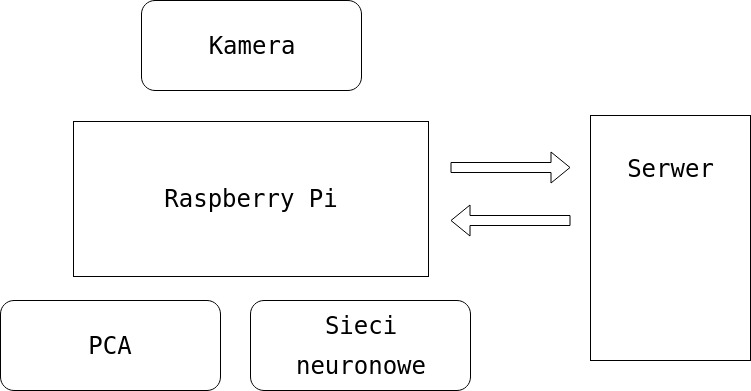
\includegraphics[width=0.50\textwidth,natwidth=610,natheight=642]{img/schemat_pogladowy.jpg}\par\vspace{0.5cm}
\caption{Schemat poglądowy działania systemu}
	\label{fig:schemat_pogl}
\end{figure}



\subsection{Wykorzystane wzorce projektowe}

W celu ułatwienia pracy współpracownikom, w projekcie został wydzielony łatwo wymienialny komponent. Dla ułatwienia pracy badawczej, komponent został podzielony na mniejsze elementy z wykorzystaniem obiektowych wzorców projektowych.
Do reprezentacji całego komponentu wybrano wzorzec "Fabryka". Zapewniono w ten sposób elastyczność użytkownikom klasy, ponieważ mogą oni zdecydować, w jaki sposób współrzędne będące wynikiem działania algorytmów mają być przechowywane. Zapewniono klasę bazową do przechowywania wektora uczącego dla sieci, po której dziedziczą poszczególne reprezentacje, takie jak bezpośrednie przechowywanie danych w pamięci programu, czy zapis w pamięci nieulotnej w postaci pliku z rozszerzeniem .npy z biblioteki numpy.
W celu zwiększenia elastyczności w obrębie komponentu, do wyboru algorytmów dwukrotnie wykorzystano wzorzec "Strategia". Stworzono klasy bazowe do reprezentacji podstawowych własności algorytmu, które następnie implementowano w klasach pochodnych. Modyfikacja ta ułatwiła pracę badawczą i usystematyzowała strukturę projektu.

\subsection{Wykorzystane zasady i dobre praktyki programowania}

W trakcie realizacji projektu, oprócz wykorzystania wzorców projektowych posługiwano się także dobrymi zasadami SOLID oraz Clean Code. Pozwalają one na zachowanie większego porządku oraz czytelności kodu. SOLID opisuje dobre praktyki programowania obiektowego i składa się z pięciu zasad:

\begin{enumerate}
\item Pojedyncza odpowiedzialność (Single resposibility)

Zasada ta zawiera się w sformuowaniu: powinien istnieć jeden i tylko jeden powód do modyfikacji klasy. Każda z klas powinna mieć tylko jedną odpowiedzialność. Pojedyncza odpowiedzialność klas umożliwia łatwiejszą modyfikację kodu i definiowanie nowych zachowań. Zasada ta prowadzi do powstania wielu klas w projekcie, jednakże przemyślane zaprojektowanie struktury klas pozwala na uniknięcie nieporządku w projekcie.

\item Otwarte/Zamknięte (Open/Closed)

Zasada ta oznacza, że należy projektować i tworzyć klasy w taki sposób, aby ich rozszerzanie było łatwe, jednocześnie nie wymagało modyfikacji już istniejącego kodu. W zachowaniu tej zasady mogą pomóc takie narzędzia jak polimorfizm, czy wzorzec projektowy constructor chaining.

\item Zasada podstawienia Liskov (Liskov substitution)

"Jeżeli q(x) jest udowadnialną własnością obiektu x typu T, to q(y) powinno być prawdziwe dla obiektu y typu S, gdzie S jest podtypem T." Zasada ta mówi, że w~dowolnym momencie klasa bazowa może się zamienić z klasą pochodną. Przestrzeganie tej zasady umożliwia stosowanie wskaźników na klasę bazową wskazujące na klasy pochodne bez jakichkolwiek obaw. Klasa pochodna zachowa się w podobny sposób do klasy bazowej, bez niepożądanych, bądź ukrytych efektów ubocznych wykonania funkcji. Najczęściej podawanym przykładem nieprzestrzegania tej zasady jest klasa Kwadrat, dziedzicząca po klasie Prostokąt. Zmiana wysokości lub długości podstawy w~klasie bazowej odpowiada jednej operacji zmiany długości boku w~klasie pochodnej, przez co jedna z operacji z klasy bazowej traci sens, a użycie klasy pochodnej w miejsce bazowej może mieć niepożądane skutki.

\item Zasada niezależności interfejsów (Interface segregation principle)

Segregacja interfejsów polega na ograniczeniu rozmiarów interfejsów. Klasy powinny implementować tylko te metody z interfejsów, które są im potrzebne. Jeśli tak nie jest, należy podzielić interfejsy na mniejsze i dać użytkownikowi możliwość dziedziczenia tylko tych potrzebnych. Przestrzeganie tej zasady pozwala na tworzenie minimalistycznego kodu, który ma wykonywać to co zakładano, a dodatkowo jest łatwy w refaktoryzacji.

\item Odwrócenie zależności (Dependency inversion)

"Wszystkie moduły powinny zależeć od abstrakcji, a nie od konkretnego typu." Wysokopoziomowe moduły nie mogą posiadać zależności do niskopoziomowych modułów. Zamiast tego oba powinny polegać na abstrakcjach. Zasada ta jest mocno powiązana z pierwszą zasadą. Jeśli każda klasa posiada tylko jedną odpowiedzialność, zdefiniowanie jasnych interfejsów między nimi jest łatwiejsze. Definiowanie abstrakcyjnych interfesjsów pozwala na jasne oddzielenie od siebie różnych komponentów i delegowanie zadań. W przestrzeganiu tej zasady pomaga taka technika jak wstrzykiwanie zależności.

\end{enumerate}

Clean Code, to zbiór zasad dotyczących tworzenia nazewnictwa i pisania oprogramowania w taki sposób, aby był on jak najbardziej czytelny dla innych programistów. Według założeń Clean Code wszystkie elementy oprogramowania takie jak klasy, struktury, funkcje, metody, obiekty, miały nazwę adekwatną do realizowanej czynności lub przeznaczenia. Dodatkowo nazwy obiektów o lokalnym zakresie i krótkim czasie życia powinny być jak najkrótsze. Nazwy obiektów o dużym zasięgu powinny być jak najdłuższe. W przypadku funkcji zasda ta jest odwrócona: projektując interfejs klasy należy udostępniać użytkownikowi jak najkrótsze nazwy. Nazwy metod prywatnych powinny być jak najdłuższe i~dokładnie opisywać za co odpowiada dana metoda. Należy pisać jak najkrótsze metody. Robert C. Martin zaleca aby miały maksymalnie 6 linijek kodu. Jedną z podstawowych zasad tej ideologi jest unikanie komentowania kodu. W założeniach Clean Code, kod powinien być napisany w taki sposób, aby używanie komentarzy było zbędne. Mówi się wręcz, że "Dobrze napisany kod czyta się jak prozę". Jednym z podstawowych założeń omawianej metodologii jest duże pokrycie kodu testami jednostkowymi. Nie zdecydowano się na wykorzystanie testów jednostkowych przy pracy nad omawianym komponentem ze względu na dynamiczny charakter projektu. Definiowanie zachowań kodu w testach jednostkowych jest czasochłonne, a częste zmiany w systemie powodują, że należałby usuwać część testów.  Ideologia Clean Code zawiera także wiele innych zasad, których stosowanie prowadzi do zwiększenia porządku i czytelności kodu. Metodyka ta cieszy się dużą popularnością wśród wielu programistów, dodatkowo niektóre firmy wymagają od swoich programistów przestrzegania zasad tej metodyki.

Dobra organizacja kodu oraz porządek ułatwiają rozwijanie projektu oraz systematyzują pracę. 

\subsection{Wykorzystane biblioteki, narzędzia i zasoby}
Projekt systemu biometrycznej kontroli dostępu został zrealizowany całkowicie w języku programowania Python. Decyzja ta była podyktowana głównie znaczącą liczbą gotowych bibliotek, które bardzo ułatwiają pracę. Wykorzystana została wersja języka 2.7.9, ponieważ biblioteki języka Python często wymagają wersji 2.7 lub wyższej. W omawianym komponencie wykorzystano biblioteki NumPy, SciPy, scikit-learn, openCV oraz Dlib.
\begin{enumerate}
\item NumPy

Jest to biblioteka, zawierająca wiele algorytmów do realizacji obliczeń numerycznych oraz implementację wielu matematycznych narzędzi związanych z algebrą liniową. Implementacja algorytmów macierzowych z NumPy cieszy się dużą popularnością, dlatego warto poświęcić czas na poznanie tej biblioteki, ponieważ stanowi ona fundament wielu innych projektów, a operacje macierzowe z jej wykorzystaniem są bardzo dobrze zoptymalizowane.

\item SciPy

SciPy jest biblioteką wykorzystywaną do obliczeń naukowych i inżynierskich. Zawiera algorytmy umożliwiające przeprowadzanie obliczeń w wielu dziedzinach, dlatego również jest wykorzystywana jako baza innych projektów. Instalacja SciPy jest prerekwizytem do instlacji scikit-learn. 

\item Scikit-learn 

Jest to biblioteka, zawierająca wiele algorytmów z dziedziny machine learning oraz pattern recognition. Jest to kluczowa biblioteka w omawianym projekcie, ponieważ dostarcza najistotniejszych narzędzi. Jej zastosowanie znacznie ułatwiło pracę.

\item OpenCv

Biblioteka ta stanowi potężny zbiór narzędzi do analizy oraz przetwarzania obrazów. Twórcy biblioteki skupiają się na działaniu w czasie rzeczywistym i zapewniają narzędzia do zrównoleglania obliczeń. Jest to znaczące udogodnienie, biorąc pod uwagę podstawową platformę sprzętową, na której był realizowany projekt. 

\item Dlib 

Dlib jest biblioteką przewidzianą głównie dla języka C++, jednakże możliwe jest także wykorzystanie jej w Pythonie. Zawiera głównie algorytmy z dziedziny Machine Learning (ML). W omawianym projekcie została wykorzystana do zbadania możliwości alternatywnych metod detekcji twarzy.

\end{enumerate}

Wszystkie wyżej wymienione biblioteki są rozpowszechniane w ramach licencji new-BSD lub 3-clause BSD, co oznacza, że wolno je wykorzystywać w celach akademickich lub komercyjnych. Zastosowanie bibliotek dostarczających zoptymalizowanych algorytmów znacznie uprościło i usystematyzowało pracę nad projektem.

Na początku pracy nad projektem podjęto próbę implementacji własnej wersji algorytmu PCA, aby lepiej zrozumieć i dokładnie prześledzić jego działanie. Algorytm ten działał poprawnie, ale ze względu na dużą kosztowność obliczeniową zdecydowano się na korzystanie z wersji udostępnionej w bibliotece scikit-learn. W trakcie późniejszych prac nad systemem znaleziono informację na temat tego, co powodowało tak wysoką złożoność obliczeniową oraz sposób na jej uniknięcie. Zagadnienie to zostało opisane w Rozdziale \ref{Realizacja algorytmu} "Realizacja algorytmu".

Diagramy i rysunki wykonano z wykorzystaniem strony draw.io. Do wszystkich zapożyczonych obrazów zostały podane źródła.

Do przeprowadzenia badań, jako bazy twarzy, wykorzystano zbiór zdjęć dostępny w~ramach biblioteki scikit-learn The Olivetti faces dataset. Posłużył on jako baza do wyznaczenia wartości własnych przestrzeni zdjęć twarzy. Informacje na temat bazy zdjęć, oraz link do strony bazy zostały podane w \cite{Olivetti faces}.


\newpage

\chapter{Implementacja algorytmów – detekcja twarzy}

Pierwszym wymaganiem, po zdolności do akwizycji obrazów, jest określenie, czy uzyskane zdjęcie przestawia twarz. W niniejszym rozdziale omówiono możliwe metody detekcji twarzy na dwuwymiarowym obrazie. Szczegółowo omówiono przyjęte rozwiązanie oraz podano uzasadnienie dlaczego zostało ono wybrane.

\section{Kaskady Haara}
Algorytm Kaskad Haara (detektor Viola-Jones) wykorzystuje serię cech do określenia, czy na zdjęciu w określonym miejscu znajduje się szukany obiekt. Cecha jest tu rozumiana jako prostokąt podzielony na części. Pod każdą z części dodawane są wartości pikseli, następnie wartości z obu obszarów są od siebie odejmowane. Koncepcja ta przypomina falkę Haara, stąd druga część nazwy algorytmu. Tak uzyskana wartość musi przekroczyć odpowiedni próg, który decyduje o tym, czy w danym miejscu rozpoznano twarz. Jak podano w \cite{Kaskada Haara}, aby móc szybciej obliczać wartości pikseli pod odpowiednim obszarem, wykorzystuje się obraz kumulacyjny (ang. integral image). Jest on zdefiniowany jako:

\begin{equation}
	ii(x,y) = \sum_{x' \leq x, y' \leq y} i(x',y')
\end{equation}

Funkcja ta przypomina dyskretną dystrybuantę dwuwymiarowej zmiennej losowej. Jej zastosowanie pozwala na obliczenie sumy jasności pod dowolnie wielkim obszarem, w~dowolnym miejscu obrazu, w stałym czasie.

\begin{figure}
\centering
	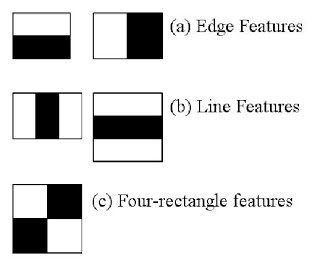
\includegraphics[width=0.50\textwidth,natwidth=610,natheight=642]{img/haar_features.jpg}\par\vspace{0.5cm}
\caption{Różne rodzaje cech}
Od sumy wartości pikseli pod czarnym obszarem jest odejmowana wartość sumy pikseli pod białym obszarem.
Źródło: https://docs.opencv.org\/3.3.0\/d7\/d8b\/tutorial\_py\_face\_detection.html
	\label{fig:features}
\end{figure}

Nawet dla najmiejsznych obrazów można rozważać wiele cech. W celu ograniczenia ilości analizowanych cech, wykorzystano alogrytm AdaBoost \cite{AdaBoost}. Algorytm ten, posiadając zbiór uczącym oraz zbiór słabych hipotez, przyporządkowywuje wagi hipotezom, oceniając ich skuteczność. Dodatkowo wagi otrzymują także przykłady ze zbioru uczącego. Każdorazowo, kiedy dany przykład zostanie źle zaklasyfikowany, jego waga jest zwiększana. 


\begin{figure}
\centering
	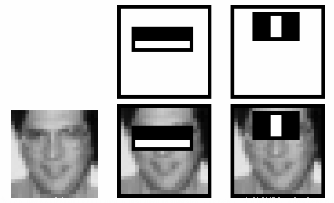
\includegraphics[width=0.50\textwidth,natwidth=610,natheight=642]{img/haar.png}\par\vspace{1cm}
\caption{Dwie cechy, generujące najmniejszy błąd z wykorzystaniem AdaBoost}
Źródło: https://docs.opencv.org\/3.3.0\/d7\/d8b\/tutorial\_py\_face\_detection.html
	\label{fig:best_features}
\end{figure}

Wykorzystanie AdaBoost pozwoliło na wybranie cech generujących najmniejszy błąd. Ilość użytych cech wpływa na jakość algorytmu, jednocześnie zwiększając czas potrzebny na obliczenia. Jak można zauważyć na Rys. \ref{fig:best_features} najlepsze cechy mają dość intuicyjną interpretację: spodziewamy się, że obraz w okolicach oczu będzie ciemniejszy niż w okolicach policzków oraz, że środek nosa będzie jaśniejszy niż obszary po bokach.

Dysponując zbiorem cech można przystąpić do klasyfikacji obrazu. Odbywa się to kaskadowo. W pierwszym etapie wykorzystuje się klasyfikator złożony najczęściej z jednej lub dwóch cech. Klasyfikacja jest przeprowadzana na całym obrazie, aby wykryć gdzie może znajdować się twarz. W kolejnych etapach ilość cech jest zwiększana (najczęściej wykładniczo). Jeśli w danym obszarze nie została wykryta twarz, zostaje on pominięty w dalszych etapach. Pozwala to znacząco ograniczyć ilość wykonywanych operacji dla kolejnych klasyfikatorów. Zaleca się, aby w pierwszym etapie wykorzystywać cechę z wysokim współczynnikiem fałszywych negatywnych rezultatów (ang. false negative) -- w tym przypadku obszarów zawierających twarz, błędnie zaklasyfikowanych jako nie będących twarzą.

Kaskady Haara są szybkie, przez co chętnie wykorzystuje się je w projektach wymagających przetwarzania obrazów w czasie rzeczywistym. Było to także motywacją przy wyborze tej metody w omawianym systemie. Rozwiązanie daje zadowalające wyniki przy jednoczesnym szybkim działaniu. W rozważanym systemie złożoność obliczeniowa musi być rozpatrywana, biorąc pod uwagę, że oryginalna platforma sprzętowa, na którą został przewidziany system to Rasbery Pi.

\section{Inne sposoby rozwiązania problemu} \label{geometrical_features}

\begin{figure}
\centering
	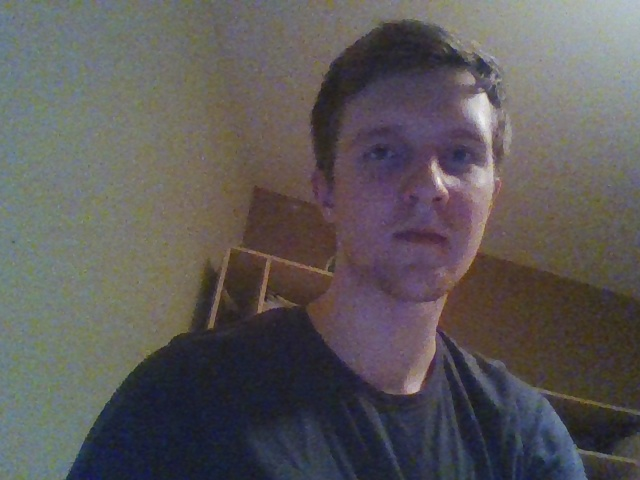
\includegraphics[width=0.40\textwidth,natwidth=310,natheight=642]{img/test.jpg}
	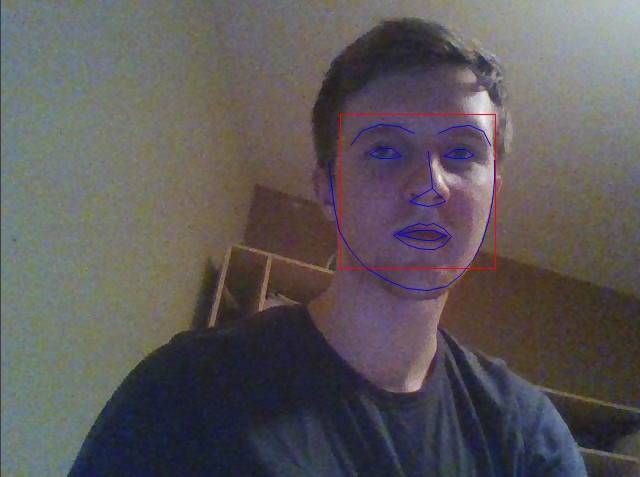
\includegraphics[width=0.40\textwidth,natwidth=310,natheight=642]{img/test_result.jpg}
\caption{Wykrywanie punktów charakterystycznych twarzy}
W lewej części - oryginalne zdjęcie, w prawej - części, obraz z zaznaczonym rezultatami detekcji. Wykrozystano 68 cech.
	\label{fig:face_landmark_detect}
\end{figure}

Do rozwiązania problemu można zastosować inne podejście, polegające na znajdowaniu charakterystycznych punktów twarzy. W pracy \cite{Landmark face detector} wykorzystano boosting drzewa gradientu do stworzenia kaskady regresorów. Dysponując zbiorem uczącym, zawierającym zdjęcia twarzy oraz współrzędne punktów charakterystycznych można wyznaczyć kaskadę regresorów liniowych. Zakładamy, że estymowany kształt punktów charakterystycznych dowolnej twarzy może być wyrażony jako kombinacja liniowa kształtu punktów charakterystycznych z odpowiednio dużego zbioru uczącego. Każdy regresor to drzewo decyzyjne, które w liściach przechowuje wektor, który powinien zostać dodany do aktualnej estymacji punktów charakterystycznych (zbiór współrzędnych x i y, które powinny być kolejno dodane do każdej współrzędnej). W pierwszym kroku jako estymacja, jest wykorzystywany średni kształt z bazy zdjęć uczących. Następnie każdy regresor delikatnie poprawia estymację, przesuwając punkty w odpowiednią stronę. Na Rys. \ref{fig:face_landmark_detect} przedstawiono efekty detekcji twarzy z wykorzystaniem implementacji z biblioteki Dlib.

Omawiane rozwiązanie umożliwia całkowicie inne podejście do problemu ekstrakcji cech. Mając estymatę, charakterystyczne punkty twarzy oraz mierząc odległości między poszczególnymi punktami, można przygotować wektor uczący, mający bardzo fizyczną interpretację. Dodając informację na temat koloru oczu, czy skóry, można skonstruować zupełnie inne wektory cech, niż proponowane w tej pracy. 

\newpage
 
\chapter{Implementacja algorytmów – ekstrakcja cech}

Niniejszy rozdział traktuje o algorytmach, umożliwiających ekstrakcję cech twarzy ze zdjęcia. Dysponując zdjęciem twarzy, należy zaproponować sposób utworzenia wektora, będącego reprezentatywnym odzwierciedleniem ilościowych cech ze zdjęcia i jednocześnie umożliwiającym sieci neuronowej dokonanie klasyfikacji. Zadanie to jest bardzo abstrakcyjne, zależy od wielu czynników i trudno jest określić rezultaty.

W rozdziale tym skupiono się głównie na podejściu, polegającym na zastosowaniu algorytmów redukcji wymiarowości, takich jak PCA, czy SVD. Jest to dość popularne rozwiązanie i w przypadku PCA można uzyskać wyniki mające wizualną interpretację, co jest bardzo pomocne przy pracy nad tego typu problemem.

Obraz, po wykryciu twarzy, jest obcinany do kwadratu, na którym ją wykryto, następnie obraz jest obcinany do rozmiaru 64 $\times$ 64 piksele, w celu ujednolicenia rozmiarów przetwarzanych obrazów oraz zwiększenia szybkości przetwarzania.
 
\section{Principle Components Analysis}

Principle Components Analysis (PCA) jest algorytmem redukcji wymiarowości danych. Mając określony zbiór obserwacji, będący reprezentatywną reprezentacją próbą analizowanej przestrzeni, należy wyznaczyć zbiór wektorów bazowych, tak aby wariancja danych ze zbioru obserwacji, względem nowo wyznaczonych wektorów bazowych, była jak największa.

\subsection{Wstęp matematyczny}

Przedstawione tu wyprowadzenie jest podawane za Pattern recognition and machine learning \cite{Pattern recognition}.

Zakładamy, że dany jest zbiór $D$-wymiarowych wektorów obserwacji: $\bb{x}_n , n \in 1,...,N $. Celem jest znalezienie nowej $M$-wymiarowej bazy ($M < D$) takiej, że wariancja zbioru wektorów $\bb{x}_n$, po zrzutowaniu na nową bazę, jest największa. W celu pokazania procesu i rozumowania przyjmijmy, że szukamy jednego wektora $\bb{u}_1$. Wektor ten, ponieważ ma stanowić bazę, musi być D-wymiarowy. Dodatkowo przyjmiemy, że wektor $\bb{u}_1$ jest jednostkowy, co zapiszemy w postaci warunku:
\begin{equation} \label{eq:wektor_jednostkowy}
	\bb{u}_1^{T}\bb{u}_1 = 1
\end{equation}

Rzut wektora \bb{x} na kierunek wyznaczany przez wektor \bb{u} jest dany przez: $u^{T}x$. Fakt ten ma proste uzasadnienie geometryczne:
\begin{align*}	
	\bb{u}^{T} \bb{x} &= \bb{u} \circ \bb{x} \\
		   & = ||\bb{u}|| ||\bb{x}|| cos \angle (\bb{u}, \bb{x}) \index{1} \\
		   &= ||\bb{x}|| cos \angle (\bb{u}, \bb{x}) \index{1} && \text{(\ref{eq:wektor_jednostkowy})}
\end{align*}

Przyjmimy średnią jako estymator wartości oczekiwanej:
\begin{equation}	\overline{\bb{x}} = \frac{1}{N} \sum_{n=1}^{N} \bb{x}_n \end{equation}

Wariancja zmiennej losowej $X$ jest dana przez:
\begin{align*}	\notag
	var[X]  &= \mathbb{E}[(X - \mathbb{E}[X])^2] \\
			&= \mathbb{E}[X^2] - \mathbb{E}[X]^2
\end{align*}

Wariancja jest miarą rozrzutu wartości zmiennej losowej. Im większe różnice między wartościami przyjmowanymi przez zmienną losową, tym większa jest wariancja.

Estymator wariancji dla próby losowej $x_n$:
\begin{equation}	\notag
	s^2 = \frac{1}{N} \sum_{n=1}^{N}(x_n - \overline{x})
\end{equation}

Kowariancja między dwoma zmiennymi losowymi jest dana wzorem:
\begin{align}	
	cov[X,Y] &= \mathbb{E}[(X - \mathbb{E}[X])(Y - \mathbb{E}[Y])]  \label{eq:cov} \\ 
			 &= \mathbb{E}[XY] - \mathbb{E}[X]\mathbb{E}[Y] \nonumber
\end{align}

Wzór ten można uogólnić dla wektorów losowych:
\begin{align*}
	cov[\textbf{X}, \bb{Y}] &= \mathbb{E}[(\bb{X} - \mathbb{E}[\bb{X}])(\bb{Y}^T - \mathbb{E}[\bb{Y}^T])] \\
							&= \mathbb{E}[\bb{X}\bb{Y}^T] - \mathbb{E}[\bb{X}]\mathbb{E}[\bb{Y}^T]
\end{align*}

Definiujemy macierz kowariancji $S$ dla zbioru obserwacji $\bb{x}_n$:
\begin{equation}
	S = \frac{1}{N} \sum_{n=1}^{N} (\bb{x}_n - \overline{\bb{x}})(\bb{x}_n - \overline{\bb{x}})^T
\end{equation}

Jak łatwo można zauważyć w powyższym wzorze, wartości oczekiwane zostały zastąpione średnimi, ponieważ nie dysponujemy rozkładami zmiennnych losowych, tylko zbiorem obserwacji.

Definiujemy wariancję zbioru obserwacji względem wektora $u_1$:
\begin{equation}
	s^2 = \frac{1}{N} \sum_{n=1}^{N}(\bb{u}_1^T \bb{x}_n - \bb{u}_1^T\overline{\bb{x}})^2 = \bb{u}_1^T S \bb{u}_1
\end{equation}

Chcąc maksymalizować wariancję $s^2$ musimy pamiętać o warunku ($\ref{eq:wektor_jednostkowy}$). Otrzymujemy więc problem optymalizacji, polegający na znalezieniu maksimum warunkowego funkcji $f(\bb{u}_1)$ z ograniczeniem $g(\bb{u}_1)$:
\begin{align*}
	f(\bb{u}_1) &= \bb{u}_1^T S \bb{u}_1 \\
	g(\bb{u}_1) &= 1 - \bb{u}_1^T \bb{u}_1 = 0
\end{align*}

Jest to problem, który można łatwo rozwiązać z wykorzystaniem mnożników Lagrange'a. W analizowanym przypadku Lagrangian przyjmuje postać:
\begin{align*}
	\mathcal{L}(\bb{u}_1, \lambda) &= f(\bb{u}_1) - \lambda g(\bb{u}_1) \\
				&= \bb{u}_1^T S \bb{u}_1 - \lambda(1 - \bb{u}_1^T \bb{u}_1)
\end{align*}

Różniczkując względem $\bb{u}_1$ i $\lambda$ oraz przyrównując do zera uzyskujemy układ równań:
\begin{align} 
\begin{cases}
	\nabla_{\bb{u}_1} \mathcal{L} (\bb{u}_1, \lambda) &= \nabla_{\bb{u}_1} \bb{u}_1^T S \bb{u}_1 - \nabla_{\bb{u}_1} \lambda \bb{u}_1^T \bb{u}_1 = 0 \\
	\frac{\partial}{\partial \lambda} \mathcal{L} (\bb{u}_1, \lambda) &= 1 - \bb{u}_1^T \bb{u}_1 = 0
\end{cases}
\end{align}

Zajmijmy się pierwszym równaniem z układu $3.6$. Odjemnik można uprościć w następujący sposób:
\begin{equation}
	\nabla_{\bb{u}_1} \lambda \bb{u}_1^T \bb{u}_1 = \lambda \nabla_{\bb{u}_1} 
		(u_{1_1}^2 + u_{1_2}^2 + ... + u_{1_D}^2)
	 	= 2 \lambda \bb{u}_1
\end{equation}

Odjemna wymaga wiecej przekształceń:
\begin{align}
	\nabla_{\bb{u}_1} \bb{u}_1^T S \bb{u}_1 
	&= \nabla_{\bb{u}_1} 
	\left( \begin{array}{llll} u_{1_1} & u_{1_2} & ... & u_{1_D} \end{array} \right)
	\begin{pmatrix}
         s_{1_1} u_{1_1} + s_{1_2} u_{1_2} + ... + s_{1_D} u_{1_D}  \\
		 s_{2_1} u_{1_1} + s_{2_2} u_{1_2} + ... + s_{2_D} u_{1_D} && \\
		 \vdots     \\
		 s_{D_1} u_{1_1} + s_{D_2} u_{1_2} + ... + s_{D_D} u_{1_D} && \\
    \end{pmatrix} \\
    &= \nabla_{\bb{u}_1} [u_{1_1} (s_{1_1} u_{1_1} + s_{1_2} u_{1_2} + ... + s_{1_D} u_{1_D})  \\
    				&+ u_{1_2} (s_{2_1} u_{1_1} + s_{2_2} u_{1_2} + ... + s_{2_D} u_{1_D}) \nonumber \\
    				&+ ... + u_{1_D} (s_{D_1} u_{1_1} + s_{D_2} u_{1_2} + ... + s_{D_D} u_{1_D})] \nonumber \\
    &= \begin{pmatrix}
    	2 s_{1_1} u_{1_1} + 2 s_{1_2} u_{1_2} + ... + 2 s_{1_D} u_{1_D}  \\
    	2 s_{2_1} u_{1_1} + 2 s_{2_2} u_{1_2} + ... + 2 s_{2_D} u_{1_D}  \\
    	\vdots     \\
	    2 s_{D_1} u_{1_1} + 2 s_{D_2} u_{1_2} + ... + 2 s_{D_D} u_{1_D}
    \end{pmatrix} \\
    &= 2 S \bb{u}_1
\end{align}

W przejściu między $(9)$, a $(10)$ korzystamy z faktu, że macierz $S$ (macierz kowariancji) jest symetryczna.

Wracając do $(3.6)$:
\begin{align} \label{eq:egienvalues}
	2 S \bb{u}_1 &- 2 \lambda \bb{u}_1 = 0	\nonumber \\
	S \bb{u}_1 &= \lambda \bb{u}_1 
\end{align}

Równość (\ref{eq:egienvalues}) jest równaniem na wartości własne macierzy $S$, więc $u_1$ musi być wektorem własnym macierzy $S$, $\lambda$ wartością własną macierzy $S$.

Mnożąc $(11)$ lewostronnie przez $u_1^T$ otrzymujemy:
\begin{equation} \label{eq:var_lambda}
	\bb{u}_1^T S \bb{u}_1 = \lambda
\end{equation}

Lewa część (\ref{eq:var_lambda}) to wariancja, która ma być maksymalizowana. Aby uzyskać jak największą wariancję zbioru obserwacji, po zrzutowaniu na kierunek wyznaczany przez $\bb{u}_1$, należy wybrać największą wartość własną macierzy S. Odpowiadający jej wektor własny jest szukanym wektorem $\bb{u}_1$. Dla kolejnych wektorów $\bb{u}$ należy znaleźć kolejne największe wartości własne i wektory własne.

\subsection{Realizacja algorytmu}  \label{Realizacja algorytmu}
Korzystając z PCA można zmniejszyć wymiarowość danych w taki sposób, aby zachować najwięcej informacji. Działanie algorytmu można zasadniczo podzielić na dwa etapy. Pierwszy, to uzyskanie bazy wektorów, która zostanie wykorzystana w drugim etapie do uzyskania nowej reprezentacji wektorów z oryginalnej przestrzeni.

W pierwszym etapie należy obliczyć wartości własne macierzy kowariancji, jak to zostało pokazane w poprzednim dziale. Przyjmijmy, że dysponujemy macierzą pomiarów:
\begin{align}
	X_{D \times N} = 
	\left( \begin{array}{llll}
		\bb{x}_1 & \bb{x}_2 & \ldots & \bb{x}_N
	\end{array} \right)	
	=
	\left( \begin{array}{llll}
		x_{1_1} & x_{1_2} & \ldots & x_{1_N} \\
		x_{2_1} & x_{2_2} & \ldots & x_{2_N} \\
		\vdots  & \vdots  & \ddots & \vdots  \\
		x_{D_1} & x_{D_2} & \ldots & x_{D_N}
	\end{array} \right)
\end{align}

Zdefiniujmy macierz A, powstałą w wyniku odjęcia od każdego wiersza średniej:
\begin{equation}
	A_{D \times N} = 
	\left( \begin{array}{llll}
	\bb{x}_1 - \overline{\bb{x}} & \bb{x}_2 - \overline{\bb{x}} & \ldots & \bb{x}_N - \overline{\bb{x}}
	\end{array} \right)
\end{equation}


Dysponując macierzą A, można zapisać S w postaci:
\begin{equation}
	S_{D \times D} = \frac{1}{N} A A^T
\end{equation}
co jest całkowicie zgodnie z definicją (\ref{eq:cov}). Kolejnym krokiem będzie wyznaczenie wektorów i wartości własnych, posortowanie wektorów własnych według nierosnącej wartości własnych oraz wybranie M wektorów własnych. 

Należy zwrócić uwagę na wymiar macierzy S. Przypomnijmy, że D to wymiar wektora pomiarowego, co w przypadku zdjęć oznacza wartość każdego piksela przeniesioną kolejno do elementów wektora. Zdjęcia w tej pracy, przed podaniem na wejście algorytmu ekstrakcji cech, były konwertowane do skali szarości i obcinane do rozmiaru 64 $\times$ 64 pikseli, co oznacza, że wektor pomiarowy zawierał 4096 współrzędnych. Biorąc pod uwagę złożoność obliczeniową algorytmów wyznaczania wektorów własnych, może to powodować problemy z wydajnością. Można temu zapobiec poprzez zamianę miejscami macierzy $A$ i $A^T$ w~iloczynie. Obliczając wartości własne macierzy $A^T A$ musimy wrócić do $D$-wymiarowości przestrzeni, co jest możliwe z wykorzystaniem następującej własności:
\begin{equation}
	u_i = A v_i
\end{equation}
gdzie $v_i$ oznacza wartość własną macierzy $A^T A$. Poprzez zamianę miejscami macierzy $A$ i~$A^T$ zyskujemy inny wymiar macierzy. Iloczyn ma teraz rozmiar NxN. Przypomnijmy, że N to liczność zbioru obserwacji. Zazwyczaj N jest znacznie niższe od D, co może przyśpieszyć obliczenia. Korzystając z tego uproszczenia należy pamiętać, że zostaje nałożone ograniczenie co do wielkości M. Jako, że zostają obliczone wektory własne macierzy o~rozmiarze NxN, może ich być maksymalnie N. Oznacza to, że ilość wymiarów danych po redukcji nie może przekraczać ilości danych ze zbioru obserwacji ($M < N$). Ograniczenie to nie jest zbyt dotkliwe, gdy dysponujemy odpowiednio wielkim zbiorem obserwacji. W~przypadku tej pracy rozmiar bazy zdjęć nie był problemem.

Po konwersji do oryginalnej wymiarowości dysponujemy bazą $M$ wektorów $D$- wymiarowych. Zbiór $M$ wektorów jest nazywany wartościami własnymi i zostanie wykorzystany w drugim etapie. Dla uproszczenia wektory własne zostaną włączone do jednej macierzy:
\begin{equation}
	U = 
	\left( \begin{array}{l}
		\bb{u}_1^T \\
		\bb{u}_2^T \\
		\vdots	 \\
		\bb{u}_M^T
	\end{array} \right)
\end{equation}
W pewnym sensie macierz $U$ wyznacza reguły, przy pomocy których konwertujemy wektory $D$-wymiarowe na $M$-wymiarowe.

Drugim etapem działania algorytmu jest redukcja wymiarowości wektora $\bb{w}$ spoza zbioru obserwacji. Obrazowo można powiedzieć, że na podstawie nowego zdjęcia, niewykorzystanego w poprzednim etapie, chcemy uzyskać reprezentujący je wektor liczb w~przestrzeni o niższym wymiarze. Odbywa się to zasadniczo w dwóch, bardzo prostych krokach: Pierwszym jest odjęcie od nowego wektora średniej. Drugim jest rzutowanie różnicy $\bb{w} - \overline{\bb{x}}$ na wcześniej uzyskane wartości własne. Uzyskanie współrzędnych w $M$-wymiarowej przestrzeni wektora $w$ można więc zapisać jako:
\begin{equation}
	\bb{v} = U ( \bb{w} - \overline{\bb{x}} ) 
\end{equation}

Z powyższego wzoru wynika, że $\overline{\bb{x}}$ oraz $U$ zależą bezpośrednio od zbioru obserwacji, jakimi dysponujemy na początku. Dobranie zbioru reprezentatywnego dla danej przestrzeni jest kluczowe. Pierwszy etap działania algorytmu, polegający na generacji wektorów własnych, definiuje przekształcenie. Drugi etap działania pozwala na redukcję wymiarowości dowolnego $D$-wymiarowego wektora zgodnie z regułami ustalonymi w pierwszym kroku.

\subsection{Interpretacja}
Warto poświęcić uwagę na to, co tak na prawdę zyskujemy w wyniku działania algorytmu PCA. Przez odjęcie średniej, przesuwamy środek nowo powstałego układu współrzędnych do punktu gdzie znajdowała się średnia zbioru obserwacji. Dodatkowo, po odjęciu średniej, wektor reprezentuje jedynie różnicę miedzy średnią (środkiem nowego układu współrzędnych), a punktem końcowym. Jest więc reprezentacją unikatowych cech w zbiorze obserwacji. Wybranie wektorów własnych, będących osiami - kierunkami z największą wariancją powoduje, że odrzucając część bazy wektorów tracimy najmniej zróżnicowane dane. W celach badawczych można wrócić do oryginalnej przestrzeni, aby porównać błąd przybliżenia oraz przeanalizować jak bardzo reprezentacyjne są uzyskane wyniki. W~przypadku zdjęć, możliwe jest wręcz wizualne porównanie jak bardzo oryginalne zdjęcie i zdjęcie odtworzone po redukcji wymiarowości są podobne do siebie. Rekonstrukcja odbywa się w następujący sposób:
\begin{equation}
	\bb{w} \approx \overline{\bb{x}} + \sum_{n=1}^{M} \bb{v}_n \bb{u}_n
\end{equation}
gdzie $\bb{v}_n$ oznacza $n$-ty element wektora $v$, a $\bb{u}_n$ oznacza $n$-ty wektor $u$.

\begin{figure}
\centering
	\parbox{2cm}{
		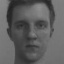
\includegraphics[width=2cm]{img/face_1.jpg}
		}
		\qquad
		\begin{minipage}{2cm}
			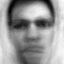
\includegraphics[width=2cm]{img/100.jpg}
		\end{minipage}
		\begin{minipage}{2cm}
			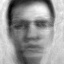
\includegraphics[width=2cm]{img/200.jpg}
		\end{minipage}
		\begin{minipage}{2cm}
			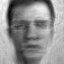
\includegraphics[width=2cm]{img/300.jpg}
		\end{minipage}
		\begin{minipage}{2cm}
			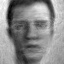
\includegraphics[width=2cm]{img/400.jpg}
		\end{minipage}
	\caption{Porównanie rekonstrukcji zdjęcia twarzy autora pracy na postawie różnej liczby wykorzystanych składowych} 
	Z lewej strony oryginalne zdjęcie, następnie kolejno rekonstrukcja z wykorzystaniem 100, 200, 300 i 400 składowych.
	\label{fig:rekonstrukcja}
\end{figure}

Efekt rekonstrukcji przedstawiono na Rys. \ref{fig:rekonstrukcja}. Dokonano redukcji wymiarowości zdjęcia twarzy autora systemu oraz na podstawie uzyskanego wektora zrekonstruowano oryginalny obraz. Wraz ze zwiększeniem się ilości składowych, jakość rekonstrukcji zdjęcia się polepsza. Użycie większej ilości składowych nie przynosi znaczącej poprawy jakości obrazu, co można zaobserwować dla rekonstrukcji z wykorzystaniem 300 i 400 składowych. PCA jest chętnie wykorzystywaną metodą, ponieważ jest bardzo intuicyjna oraz pozwala na wizualne sprawdzenie rezultatów.

\begin{figure}
\centering
	\parbox{2cm}{
		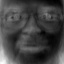
\includegraphics[width=2cm]{img/0.jpg}
		}
	\begin{minipage}{2cm}
		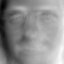
\includegraphics[width=2cm]{img/1.jpg}
	\end{minipage}
	\begin{minipage}{2cm}
		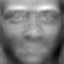
\includegraphics[width=2cm]{img/2.jpg}
	\end{minipage}
	\begin{minipage}{2cm}
		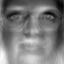
\includegraphics[width=2cm]{img/3.jpg}
	\end{minipage}
	\begin{minipage}{2cm}
		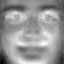
\includegraphics[width=2cm]{img/4.jpg}
	\end{minipage}\\
	
	\begin{minipage}{2cm}
		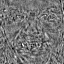
\includegraphics[width=2cm]{img/392.jpg}
	\end{minipage}
	\begin{minipage}{2cm}
		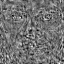
\includegraphics[width=2cm]{img/393.jpg}
	\end{minipage}
	\begin{minipage}{2cm}
		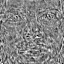
\includegraphics[width=2cm]{img/394.jpg}
	\end{minipage}
	\begin{minipage}{2cm}
		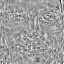
\includegraphics[width=2cm]{img/395.jpg}
	\end{minipage}
	\begin{minipage}{2cm}
		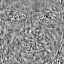
\includegraphics[width=2cm]{img/396.jpg}
	\end{minipage}
	\caption{Porównanie eigenfaces}
Górny wiersz - wektory 0-4, dolny wiersz - wektory 392-396.
	\label{fig:eigenfaces}
\end{figure}

W omawianym zagadnieniu wektory własne zyskały specjalną nazwę eigenfaces (twarze własne), można zauwżyć jak wyglądają aplikując technikę odtwarzania zdjęcia na podstawie współrzędnych z przestrzeni o zredukowanej wymiarowości. Efekty zostały zaprezentowane na Rys. \ref{fig:eigenfaces}. 

Z rysunku jednoznacznie wynika, że wektory 0-4 zawierają najbardziej istotne zmiany pomiędzy poszczególnymi obrazami ze zbioru obserwacji - odpowiadają one wartościom własnym o największej wariancji. Wektory 392-396 odpowiadają niższym wartościom własnym. Wektory te przypominają losowy szum i niosą informację o szczegółach twarzy. Można zauważyć, że pominięcie składowych z niższą wartością własną, powoduje mniejszą utratę informacji - dane w kierunkach wyznaczanych przez te wektory nie różnią się znacząco od siebie.

\subsection{PCA jako samodzielny system rozpoznawania twarzy}
Principle components analysis powoduje przeniesienie zdjęcia, mającego wizualną reprezentację na abstrakcyjny wektor liczb. Umożliwia to skonstruowanie klasyfikatora z wykorzystaniem algorytmów klasyfikacji. Jest to zagadnienie dobrze znane w dziedzinie Pattern Recognition (rozpoznawania wzorców) i opracowano wiele rozwiązań tego problemu. Zastosowanie algorytmów typu k-NN (k Nearest Neighbour - k najbliższych sąsiadów) lub NM (Nearest Mean - najbliższa średnia) umożliwia zaklasyfikowanie danego algorytmu do jednej z grup. Jest to możliwe dzięki wykorzystaniu reprezentacji zdjęcia jako wektora liczb. Oba algorytmy dysponują zbiorem uczącym, który opisuje dane grupy, do których może zostać klasyfikowany dany wzorzec. 
W przypadku NM, dla każdej z grup, obliczana jest średnia wektorów, następnie obliczana jest odległość między wektorem podlegającym klasyfikacji, a średnimi zbiorów. Wektor zostaje zaklasyfikowany do zbioru, którego średnia jest w najmniejszej odległości od wektora. 
W przypadku algorytmu k-NN, odległość jest obliczana pomiędzy wszystkimi wektorami ze zbioru uczącego. Następnie zostaje wybrane k najbliższych sąsiadów. Zbiór, którego najwięcej przedstawicieli zostało wybranych wygrywa. Dla przypadku dychotomii, jeżeli k jest nieparzyste, to możliwa jest jednoznaczna klasyfikacja. Gdy ilość zbiorów, do których można zaklasyfikować obraz jest większa od dwóch, możliwe jest wystąpienie wypadku, w którym nie można jednoznacznie zaklasyfikować obiektu. 
W przypadku systemu kontroli dostępu może być wskazane wprowadzenie maksymalnej odległości między średnią lub najbliższym sąsiadem, a analizowanym wektorem. Powyżej tej odległości obraz nie powinien być zaklasyfikowany do którejkolwiek z~grup. 
Dodatkowo warto zwrócić uwagę na brak kontroli PCA nad przetwarzanymi danymi. Zdjęcie przetwarzane przez metodę statystyczną, może przedstawiać mysz lub samochód i zostanie podany wynik. Nie wiadomo jakie współrzędne można uzyskać dzięki takiej operacji, ani jak zostaną zinterpretowane wyniki przez system. Algorytm rozpoznawania twarzy powinien odrzucić takie zdjęcie na etapie wykrywania obecności twarzy.

\section{Inne podejścia do problemu redukcji wymiarowości}
Istnieje wiele algorytmów umożliwiających redukcję wymiarowości. Ze względu na rosnącą ilość danych do przetwarzania, algorytmy te zyskały na znaczeniu. W niniejszym fragmencie pracy zostaną krótko omówione zasady działania trzech algorytmów umożliwiających redukcję wymiarowości.

\subsection{Nonnegative Matrix Factorization}

Nonnegative Matrix Factorization (NMF) jest sposobem rozkładu macierzy na dwie mniejsze. Przyjmimy, że dana jest macierz $V_{m \times n}$, która ma zostać poddana redukcji wymiarowości. Macierz ta zostaje wyrażona jako iloczyn dwóch mniejszych macierzy:

\begin{equation}
	V \approx WH
\label{NMF}
\end{equation}

Zakłada się rozmiary macierzy: $W_{m \times k}$ oraz $H_{k \times n}$, dla $k \leq min(m,n)$. Dodatkowo przyjmuje się, że zarówno $W$, jak i $H$ są nieujemne. Wynika z tego, że stosując taki zapis i przyjmując stosunkowo małą wartość $k$, można zapisać $V$ z wykorzystaniem mniejszej ilości zmiennych. Ponadto korzystając ze spostrzeżenia, że wektory kolumnowe $V$ mogą zostać zapisane jako:

\begin{equation}
	\bb{v}_i = W \bb{h}_i,
\end{equation}

można przyjąć W, jako bazę przestrzeni definiowanej przez $V$.

Dokładny rozkład we wzorze (\ref{NMF}) nie musi istnieć dla dowolnego $k$, dlatego nie może zostać umieszczony znak równości. Zwykle w trakcie wyznaczania $W$ i $H$ przyjmuje się, że ich iloczyn ma się znajdować w odpowiednio niewielkiej odległości od $V$. Najczęściej rozważane wartości błędu to:

\begin{align*}
	||A - B||^2 &= \sum_{ij} (A_{ij} - B_{ij})^2 \\
	  D(A||B)   &= \sum_{ij} (A_{ij} log \frac{A_{ij}}{B_{ij}} - A_{ij} + B_{ij})
\end{align*}

Pierwsze równanie to znana norma L2, czyli odległość Euklidesowa. Drugie równanie to zmodyfikowana wersja dywergencji Kullbacka-Leiblera dla nieujemnych macierzy. Jest to wielkość informująca nas o tym jak wiele informacji tracimy korzystając z estymacji $B$ rozkładu $A$. Wielkość ta nie jest normą, ponieważ nie jest symetryczna.

W pracy \cite{NMF} zaproponowano iteracyjne metody znajdowania $W$ i $H$ dla obu miar błędu. Polegały one na stopniowym poprawianiu wartości obu macierzy. Pierwszy rodzaj polegał na przemnażaniu aktualnej wartości $W$ i $H$ przez odpowiednie współczynniki, drugi rodzaj opierał się na dodawaniu odpowiedniej poprawki (rozwiązanie przypominające wyznaczanie optimum funkcji z wykorzystaniem gradientu). W obu przypadkach początkowe wartości były losowe, co powodowało, że rezultaty uzyskiwane przez algorytm mogły być różne dla tej samej macierzy $V$. Dodatkowym ryzykiem jest utknięcie w~minimum lokalnym.

W pracy \cite{NMF_SVD} zaproponowano metodę wyznaczania $W$ i $H$, która nie inicjalizuje losowo wartości początkowych, tylko korzysta z rozkładu SVD (singular-value decomposition - rozkład według wartości osobliwych), który dla macierzy $A$ o wartościach rzeczywistych zapisujemy jako:

\begin{equation}
	A = U \Sigma V^T
\end{equation}

$U$ oraz $V$ są ortogonalne, a $\Sigma$ jest macierzą diagonalną, na przekątnej, której leżą tzw. wartości osobliwe. Wektory kolumnowe $U$ są nazywane lewymi wektorami osobliwymi, wektory $V$ są nazywane prawymi wektorami osobliwymi. Autorzy \cite{NMF_SVD} wykorzystali lewe i prawe wektory osobliwe, odpowiadające największym wartościom osobliwym $\Sigma$ do inicjalizacji $W$ i $H$. Umożliwiło to poprawienie wyników oraz uzyskanie algorytmu, dającego te same rezultaty dla takiego samego wejścia. Dodatkowo czas działania programu, korzystającego z tej metody stał się bardziej deterministyczny.

\subsection{Independent Components Analysis}

Rozważmy następujący problem: dana jest obserwacja $x$, będąca liniową kombinacją wielu sygnałów $s$ o niegaussowskim rozkładzie:

\begin{equation}
	x_j = a_{j1} s_1 + a_{j2} s_2 + ... + a_{jn} s_m
\end{equation}

Powższe równanie opisuje wartość $j$-tej obserwacji. Zarówno $x$ jak i $s$ są $n$-wymiarowymi wektorami. Zapis może zostać uogólniony przez zapis macierzowy:

\begin{equation}
	\bb{x} = A \bb{s}
	\label{ICA model}
\end{equation}

$A_{n \times n}$ jest nazywane macierzą mieszania (ang. mixing matrix), $\bb{s}$ jest nazywane nieznależną składową. Celem jest odzyskanie niezależnych składowych $\bb{s}$ na podstawie $\bb{x}$.~Zauważmy, że: $\bb{s} = A^{-1}\bb{x} = W \bb{x}$. $W$ jest nazywana macierzą rozdzielania (ang. unmixing matrix). 

W celu lepszego zrozumienia opisywanego podejścia, można sobie wyobrazić, że problem ten występuje w kontekście analizy sygnału mowy: dysponujemy sygnałem, w którym wielu ludzi mówi jednocześnie, a chcemy uzyskać osobne wypowiedzi poszczególnych osób (problem cocktail party). 

W \cite{ICA} podano rozwiązanie problemu, opierające się na centralnym twierdzeniu granicznym:

Załóżmy, że wartość oczekiwana $\bb{x}$ i $\bb{s}$ jest równa 0 oraz wariancja niezależnych składowych jest równa 1. Możemy to zrobić, ponieważ dla rozkładów o niezerowej średniej można odjąć średnią. Ograniczenie nałożone na wariację $\bb{s}$ jest spowodowane przez równanie (\ref{ICA model}), konkretniej, wartość $\bb{s}$ może zostać obliczona z dokładnością do stałej ($\bb{s}$~może zostać przemnożone przez dowolne $p$, jeśli $A$ zostanie przemnożone przez $\frac{1}{p}$). Stosując to ograniczenie unikamy zbyt wielkich wartości niezależnych składowych  Dodatkowo załóżmy, że wszystkie niezależne składowe $\bb{s}$ mają taki sam rozkład i są niezależnymi zmiennymi losowymi. Wprowadźmy $\bb{y}$ jako liniową kombinację $\bb{x}$:

\begin{equation}
	\bb{y} = \bb{w}^T \bb{x}
\end{equation}

Jeśli $\bb{w}$ jest fragmentem macierzy $W$, to $\bb{y}$ musi odpowiadać jednej z niezależnych składowych. Nie możemy bezpośrednio wyznaczyć $\bb{y}$, ponieważ nie znamy $A$ i $\bb{s}$, możemy co najwyżej je estymować. Przyjmijmy:

\begin{equation}
	\bb{z} = A^T \bb{w}
\end{equation}

Wykorzystując nową zmienną możemy zapisać:

\begin{equation}
	\bb{y} = \bb{w}^T \bb{x} = \bb{w}^T A \bb{s} = \bb{z}^T \bb{s} 
\end{equation}

Możemy zauważyć, że $y$ jest kombinacją liniową \bb{s}. Zgodnie z centralnym twierdzeniem granicznym, suma dowolnych rozkładów prawdopodobieństwa dąży do rozkładu Gaussa, jeśli jest spełniony warunek Lindeberga, a w szczególności gdy $E[X] = 0$ i $\sum_{k=1}^{n}var[X] = 1$ to:

\begin{equation}
	\sum_{k=1}^{n} X_k \to N(0,1)
\end{equation}

Widzimy więc, że $\bb{y}$ będące kombinacją liniową wektorów $\bb{s}$, będzie bardziej "gaussowskie", niż dowolna z niezależnych składowych osobno. Założyliśmy, że $s$ nie ma rozkładu Gaussa więc $\bb{y}$ będzie równe $\bb{s}$, gdy będzie najmniej gaussowskie, co jest jednoznaczne z~tylko jedną, niezerową wartością w wektorze $\bb{z}$.

Autorzy \cite{ICA} proponują miary niegaussowskości oparte na kurtozie, bądź ujemnej entropii. Negatywna entropia może być dość dobrym estymatorem stopnia, w jakim rozkład nie jest gaussowski. Jest nieujemna i równa zero tylko dla rozkładu Gaussa.


Oprócz zastosowania w analizie mowy, często podawaną aplikacją ICA jest ocenianie aktywności mózgu w poszczególnych obszarach na podstawie sygnałów z elektrod rozmieszczonych w różnych miejscach głowy. W kontekście tej pracy, znalezienie wektorów $s$,~mogących definiować bazę nowej przestrzeni prowadzi do redukcji wymiarowowści danych.

\newpage


\chapter{Omówienie implementacji}

W tym rozdziale przedstawiono szczegóły implementacji kodu, realizującego omawiane funkcjonalności komponentu. Omówiono podstawowe koncepcje i założenia, kryjące się za przyjętymi rozwiązaniami. Omówiono funkcjonalności oraz zakres odpowiedzialności poszczególnych klas.

\section{Klasa zarządzająca komponentem}

W najnowszej wersji projektu najważniejszą klasą w omawianym komponencie jest AbstractFactory. Wzorzec projektowy Fabryki Abstrakcyjnej dobrze oddaje działanie komponentu z punktu widzenia reszty systemu, choć biorąc pod uwagę zakres odpowiedzialności klasy, odpowiedni jest także wzorzec Budowniczy. Jest to klasa zawierająca wszystkie niezbędne algorytmy, które są wykorzystywane przy procesach wykrywania twarzy i ekstrakcji cech. Zadaniem tej klasy jest przykrycie wszystkich zależności i szczegółów związanych z operacją przekształcania zdjęcia w wektor liczb. Efektem tej operacji jest zwrócenie obiektu Product, omówionego w późniejszej części tego rozdziału.

\subsection{Interfejs do komunikacji z resztą systemu}

W obiektowych językach programowania często można spotkać się z podziałem metod na publiczne i prywatne. Podział ten wymusza dobre praktyki na programistach, ale ma jeden bardzo praktyczny aspekt. Wszystkie metody publiczne klasy to interfejs jaki zostaje udostępniony użytkownikowi. Jest to dość naturalny podział - do interfejsu klasy zaliczają się te metody, z których może skorzystać użytkownik. W języku Python nie przewidziano podziału na metody prywatne i publiczne. Wszystkie metody klasy są publiczne z założenia. Powoduje to brak jasno określonego interfejsu klasy. W najnowszej wersji komponentu, klasa AbstractFactory, jako interfejs udostępnia metodę:

\begin{lstlisting}[language=Python]
    def fabricate(self, img_filename):
        prod = self.productType(self.n_dim)
        prod.set(self.compute_coor(self\
        .detect_face(img_filename)))
        return prod
\end{lstlisting}

Jest to metoda pozwalająca na przeprowadzanie całego procesu detekcji twarzy i ekstrakcji cech. Jako arguemnt przyjmuje nazwę pliku ze zdjęciem, a zwraca produkt.

\subsection{Konstruktor}

Dobór algorytmów, wykorzystywanych w tej klasie oraz typ zwracanego produktu jest wybierany przez użytkownika poprzez wstrzykiwanie zależności w argumentach konstruktora.

\begin{lstlisting}[language=Python]
    def __init__(self, FeatureExtractionStrategy, \
    FaceDetectionStrategy, CoordinatesProduct):
        self.n_dim = 4096
        self.n_components = 400
        self.face_detection_strategy = FaceDetectionStrategy()
        self.extraction_strategy = \
        FeatureExtractionStrategy(self.n_dim, self.n_components)
        self.productType = CoordinatesProduct
\end{lstlisting}

Użytkownik klasy przy tworzeniu obiektu typu AbstractFactory podaje w argumentach konstruktora, jakie warianty klas do detekcji twarzy, ekstrakcji cech oraz przechowywania informacji na temat produktu powinny zostać wykorzystywane. Dodatkowo w~konstruktorze rozmiary wektora przed i po redukcji wymiarowości są inicjalizowane stałymi. Wartości te wynoszą odpowiednio 4096 i 400. Pierwsza z tych wartości odpowiada rozmiarowi obrazka 64$\times$64 piksele i została przyjęta w celu dopasowania rozmiarów przetwarzanych wektorów do tych ze zbioru Olivetti faces dataset. Druga wartość jest efektem eksperymentów z siecią neuronową -- dla 400-elementowych wektorów uzyskiwano najlepsze rezultaty. Wartości te nie powinny być przyjęte jako stałe i użytkownik powinien mieć możliwość zmiany tych wartości, nie jest to jednakże rażące niedopatrzenie.

\subsection{Pozostałe funkcje}

Pozostałe dwie funkcje klasy służą do wywoływania operacji detekcji twarzy i ekstracji cech z odpowiednich strategii.

\begin{lstlisting}[language=Python]
    def detect_face(self, img_filename):
        return self.face_detection_strategy\
        .detect_face_proxy(img_filename)

    def compute_coor(self, img):
        return self.extraction_strategy.extract_features(img)
\end{lstlisting}



\section{Klasa przechowująca wyniki działania Fabryki}

Zadaniem klasy CoordinatesProduct jest nałożenie abstrakcji na sposób przechowania wektora liczb zwracanego przez AbstractFactory. Posiada dwie metody: getter i setter. Po klasie tej dziedziczą: CoordinatesProductOnDisc i CoordinatesProductInClass. Każda z nich przechowuje wektor liczb w inny sposób: pierwsza na dysku, druga bezpośrednio w~pamięci programu, jako wektor z biblioteki NumPy. Możliwość przechowywania wartości na dysku pozwala na łatwy sposób debugowania aplikacji i analizę uzyskanych danych. O~wiele prostszym rozwiązaniem mogłoby być wykorzystanie struktury danych podawanej sieci neuronowej, ale jednym z celów zastosowania CoordinatesProduct jest uniezależnienie wyników, zwracanych przez AbstractFactory od frameworku, używanego do uczenia sieci neurowej.

\section{Strategia detekcji twarzy}

FaceDetectionStrategy jest klasą abstrakcyjną, po której mają dziedziczyć wszystkie implementacje algorytmów detekcji twarzy. Zawiera metody ogólnego przeznacznia, które mogą być wykorzystywane przez klasy potomne. Do metod tych zaliczają się:

Funkcja do wczytywania obrazu i konwertowania go do skali szarości:

\begin{lstlisting}[language=Python]
	read_image_and_convert_to_greyscale(self, filename)
\end{lstlisting}

Funckja do wycinania wybranego obszaru z obrazu:

\begin{lstlisting}[language=Python]
	crop_img(self, image, x, y, w, h)
\end{lstlisting}

Funkcja do wyświetlania obrazu, w celu łatwiejszego analizowania działania aplikacji:

\begin{lstlisting}[language=Python]
	debug_show(self, img)
\end{lstlisting}

Klasa ta posiada metodę łączącą wszystkie operacje wykonywane w ramach działania algorytmu wykrywania twarzy:

\begin{lstlisting}[language=Python]
    def detect_face_proxy(self, input_img_filename, \
    output_img_filename=None):
        grayscale_image = self.\
        read_image_and_convert_to_greyscale(input_img_filename)
        (x, y, w, h) = self.detect_face(grayscale_image)
        resized_face = self.crop_img(grayscale_image, x, y, w, h)
        if output_img_filename != None:
        	self.debug_show(resized_face)
            cv2.imwrite(output_img_filename, resized_face)
        return resized_face
\end{lstlisting}

Podanie do metody dodatkowego parametru w postaci ścieżki i nazywy pliku do zapisania umożliwia łatwe debugowanie aplikacji. Metoda ta jest wywoływana w detect\_face w AbstractFactory.

Klasa HaarCascadesStrategy dziedziczy po FaceDetectionStrategy i implementuje detekcje twarzy z wykorzystaniem implementacji z biblioteki OpenCv. Kiedy na zdjęciu nie zostanie znaleziona twarz, zostanie zgłoszony wyjątek: Found 0 faces!

\section{Strategia ekstrakcji cech}

Zasada działania FeatureExtractionStrategy jest bardzo podobna do poprzedniej klasy. Stanowi ona klasę bezową dla wszystkich implementacji redukcji cech. W jej skład wchodzą metody pomocnicze, takie jak:

Funkcja do ładowania obrazu z dysku:

\begin{lstlisting}[language=Python]
	load_img(self, name)
\end{lstlisting}

Funkcja do konwertowania obrazka, wczytanego przez OpenCv na wektor NumPy:

\begin{lstlisting}[language=Python]
	convert_image_to_vector(self, img)
\end{lstlisting}

Funkcja do wczytywania plików z rozszerzeniem .npy: 
	
\begin{lstlisting}[language=Python]
	load_matrix(self, name)
\end{lstlisting}

Klasa ta udostępnia jako interfejs metodę:

\begin{lstlisting}[language=Python]
	extract_features(self, img)
\end{lstlisting}

Klasa PCA dziedziczy po FeatureExtractionStrategy. PCA przeprowadza redukcję wymiarowości z wykorzystaniem pliku eig.npy. Plik ten zawiera wszystkie wektory własne potrzebne do redukcji wymiarowości. Dodatkowo PCA wczytuje średni obraz ze zbioru obserwacji i konwertuje go do wektora. Operacja ekstrakcji cech przebiega w następujący sposób:

\begin{lstlisting}[language=Python]
    def scale_vector(self, vec):
        scaleVec = ScaleVector()
        return scaleVec.scale_vector(vec)

    def extract_features(self, img):
        vec = self.image_to_vector(img)
        scaled_vec = self.scale_vector(vec)
        mean_substracted_vec = scaled_vec - self.mean
        coordinates = np.zeros((self.n_components))
        for i in range(0,self.n_components):
            coordinates[i] = np.dot(self.components[i,:],\
            mean_substracted_vec)
        return coordinates
\end{lstlisting}

W klasie PCA wykorzystano klasę ScaleVector, odpowiedzialną za skalowanie wektora, tak aby przyjmował wartości od zera do 255:

\begin{lstlisting}[language=Python]
    def move_values(self, x, xmin, xmax, max):
        return max*(x-xmin)/(xmax-xmin)

    def scale_vector(self, vec):
        min_ = self.find_min(vec)
        max_ = self.find_max(vec)
        for i in range(len(vec)):
            vec[i] = self.move_values(vec[i], min_, max_,255.0)
        return vec

\end{lstlisting}

\section{Pozostała część oprogramowania}
Przedstawione wcześniej klasy stanowią całość komponentu, działającego w systemie. Nie jest to jednakże cały kod, jaki został sporządzony w trakcie realizacji projektu. Wyznaczanie wektorów własnych oraz skrypty, umożliwiające rekonstrukcję zdjęć na podstawie uzyskanych współrzędnych, odgrywały bardzo ważną rolę przy powstawaniu systemu. Nie zostały one włączone bezpośrednio do kodu komponentu, ponieważ są one tam zbędne. Po obliczeniu wektrów własnych dla PCA są one zapisywane w pliku z rozszerzeniem .npy, z którego następnie korzysta klasa PCA, w trakcie działania systemu. Obecny wygląd komponentu jest efektem wielu prób i błędów, testowania możliwości, jakie oferują wykorzystane biblioteki oraz wieloma poprawkami na przestrzeni życia całego projektu.

\begin{figure}
\centering
	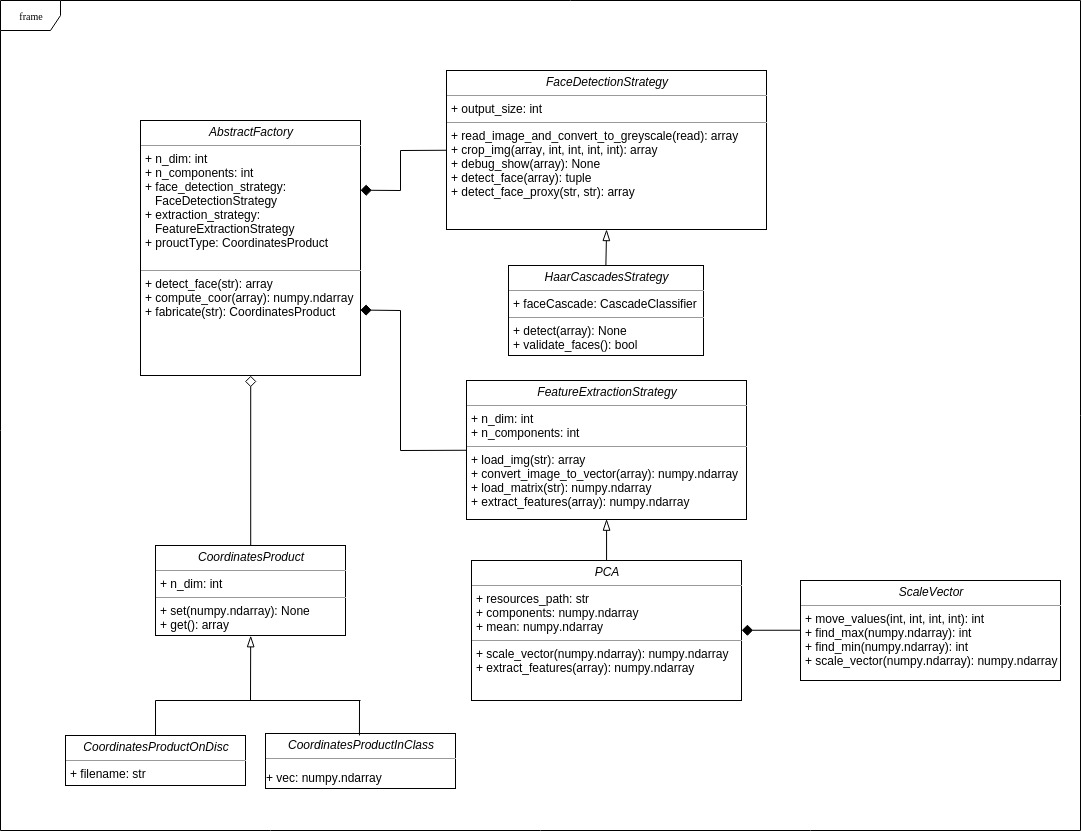
\includegraphics[width=0.90\textwidth]{img/Diagram.jpg}\par\vspace{1cm}
\caption{Diagram klas wkorzystywanych w komponencie}
	\label{fig:diagram_klas}
\end{figure}


\newpage

\chapter{Zabezpieczenie przed możliwością oszukania systemu}

W trakcie realizacji projektu specjalnościowego, jako zadanie dodatkowe zbadano jakie możliwości może dać dołączenie do systemu ekstrakcji głębi. Był to dodatek mający wskazać możliwe strony rozwoju całego projektu przy jednoczesnej próbie zaadresowania kwestii bezpieczeństwa. W trakcie testów odkryto, że istnieje możliwość oszukania całego systemu poprzez podsunięcie przed kamerę zdjęć ludzi, którym wcześniej przyznano prawo dostępu. Jest to realne zagrożenie, z którym twórcy systemów biometrycznych muszą się mierzyć. Dobrym przykładem może być tu system FaceID w IphoneX firmy Apple. Twórcy FaceID zapewniali, że nie da się go oszukać poprzez wykonanie masek 3d, imitujących twarz człowieka. W dniu 9 listopada 2017 roku, eksperci z firmy Bkav oświadczyli, że udało im się złamać zabezpieczenia poprzez wykonanie specjalnej maski z wykorzystaniem drukarki 3D, silikonowych elementów, wydruków 2D oraz materiału imitującego skórę \cite{FaceID hacked}. Dodatkowo system FaceID okazał się nie być odpornym na podobieństwo, występujące między bliźniakami jednojajowymi. Bezpieczeństwo systemów biometrycznych jest więc bardzo ważną kwestią i podjęto próbę zbadania zagadnień z~nim związanych.

\section{Przyjęta metodyka}
Zbadano możliwości, jakie daje ekstrakcja głębi z wykorzystaniem dwóch kamer. W obecnym projekcie systemu, zintegrowanie systemu ekstrakcji głębi byłoby trudne, ponieważ w projekcie wykorzystywana jest kamera Rasbery Pi, podłączona przez port CSI, a mikrokomputery Rasbery Pi posiadają tylko jeden port CSI. Do badań wykorzystano dwie kamery internetowe Creative VF0770. Do ekstrakcji głębi wykorzystano funkcje biblioteki OpenCV. Celem było uzyskanie mapy punktów w 3D, które później miały być aproksymowane płaszczyzną. Następnie należało wyznaczyć błąd aproksymacji, oraz próg, od którego mapa punktów miała być uznawana za płaską.

\section{Podstawy teoretyczne}

Przed przedstawieniem wyników omówiono przyjęte założenia teoretyczne. W nimniejszej sekcji zostały omówione takie koncepcje jak pinhole camera model, model zniekształceń w~bibliotece OpenCv, podstawowe założenia geometrii epipolarnej oraz wyznaczanie mapy głębokości na podstawie dysparycji.

\subsubsection{Model kamery}
Przed przystąpieniem do ekstrakcji głębi należy ustalić model działania pojedynczej kamery oraz zrozumieć, jakie zakłócenia obrazu występują.

\begin{figure}
\centering
	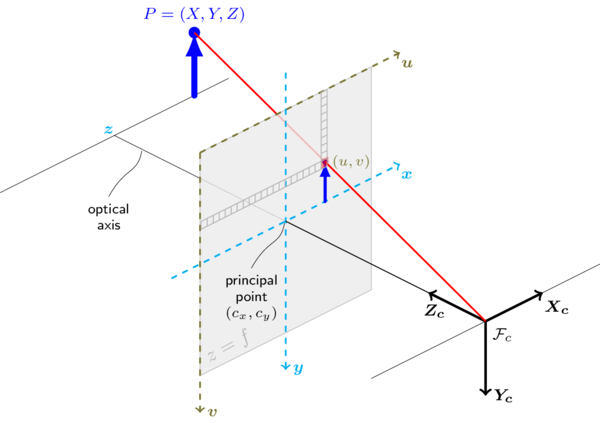
\includegraphics[width=0.90\textwidth]{img/pinhole_camera_model.png}\par\vspace{1cm}
\caption{Scena przy przyjętym modelu kamery}
Źródło: https://docs.opencv.org/2.4/modules/calib3d/doc/camera\_calibration\_and\\\_3d\_reconstruction.html
	\label{fig:camera_model}
\end{figure}

Najbardziej rozpowszechnionym modelem jest tzw. pinhole camera model. W modelu tym kamera przekształca piksele z globalnego układu współrzędnych do układu współrzednych na płaszczyźnie, na którą są rzutowane punkty. Przekształcenie to można wyrazić wzorem:

\begin{equation}
	Z
	\left( \begin{array}{l}
		u \\
		v 
	\end{array} \right) 
	= K (R \quad T) 
	\left( \begin{array}{l}
		X \\	Y \\	Z \\	1
	\end{array} \right) 
\end{equation}

W powyższym równaniu $X, Y$ oraz $Z$, to współrzędne punktu w zewnętrznym układzie współrzędnych,
$u$ i $v$, to współrzędne w układzie kamery.
Macierz R i wektor T, to macierz rotacji i wektor translacji, opisujące orientację i położenie kamery względem zewnętrznego układu współrzędnych. Zaliczają się one do parametrów zewnętrznych, ponieważ nie zależą od samej kamery, ale od jej położenia i orientacji. Parametry te opisują transformację punktu z globalnego układu współrzędnych do układu współrzędnych kamery. 

\begin{align*}
	\left( \begin{array}{l} x \\ y \\ z \end{array} \right) =
	(R \quad T)
	\left( \begin{array}{l}
		X \\	Y \\	Z \\	1
	\end{array} \right) 
\end{align*}
gdzie $x, y, z$, to współrzędne punktu P w układzie kamery.


\begin{figure}
\centering
	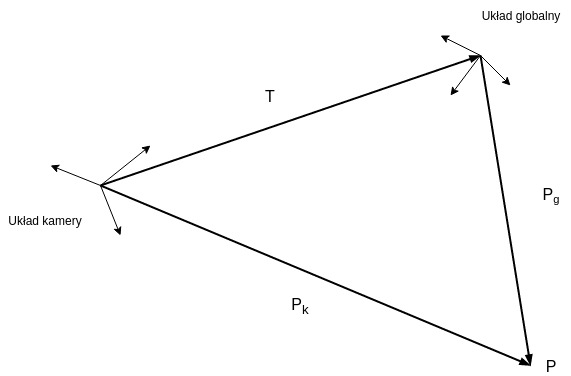
\includegraphics[width=0.90\textwidth]{img/pinhole.jpg}\par\vspace{1cm}
\caption{Ilustracja zależności między układami współrzędnych a punktem}
	\label{fig:camera_coordinate_systems}
\end{figure}

Warto zwrócić uwagę, że wektor $T$ zawiera położenie globalnego układu współrzędnych względem układu współrzędnych kamery, a nie odwrotnie. Fakt ten może wydawać się nieco nieintuicyjny, ale można go łatwo zilustrować. Z (\ref{fig:camera_coordinate_systems}) wynika jednoznacznie, że $P_k = T + P_g$. Oczywiście należy uwzględnić wzajmeną orientację układów, co zapewnia macierz R.

Macierz K zawiera parametry wewnętrzne kamery i jest definiowana jako:
\begin{equation}
	K = \left( \begin{array}{lll}
		f & 0 & c_x \\
		0 & f & c_y \\
		0 & 0 & 1
	\end{array} \right)
\end{equation}
gdzie $f$, to długość ogniskowej, $c_x, c_y$ jest punktem, w którym oś optyczna przecina się z~płaszczyzną obrazu (ang. principal point), zwykle znajdującym się w środku obrazu.

Korzystając z wcześniejszych równań można zapisać:

\begin{align*}
	u = f \frac{x}{z} + c_x \\
	v = f \frac{y}{z} + c_y
\end{align*}

\begin{figure}
\centering
	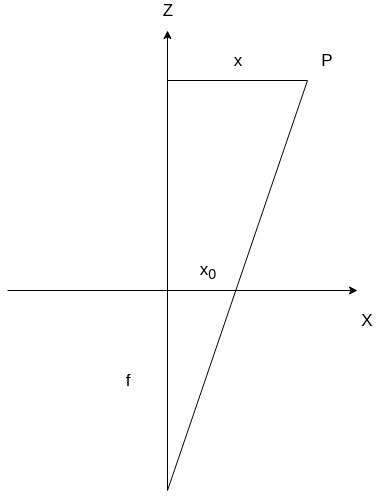
\includegraphics[width=0.50\textwidth]{img/rzutowanie.jpg}\par\vspace{1cm}
\caption{Rzut z góry na scenę}
	\label{fig:projection_up}
\end{figure}

Na rys (\ref{fig:projection_up}) można zauważyć, że równania te mają proste uzasadnienie geometryczne. Z twierdzenia Talesa otrzymujemy: 
$\frac{x_0}{f} = \frac{x}{z}$. Wartość $u$ możemy uzyskać poprzez dodanie do $x_0$ $c_x$ z poprzedniego równania. Dla y rozumowanie jest analogiczne.


\subsubsection{Zakłócenia}

\begin{figure}
\centering
		\begin{minipage}{3cm}
			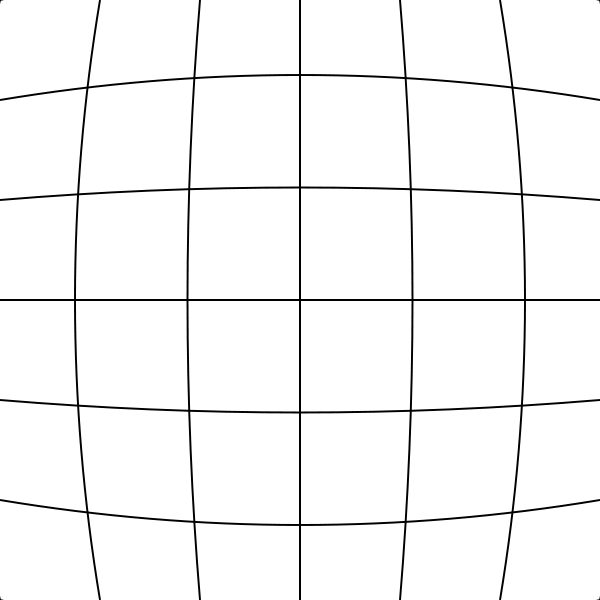
\includegraphics[width=3cm]{img/600px-Barrel_distortion.png}
		\end{minipage}
		\begin{minipage}{3cm}
			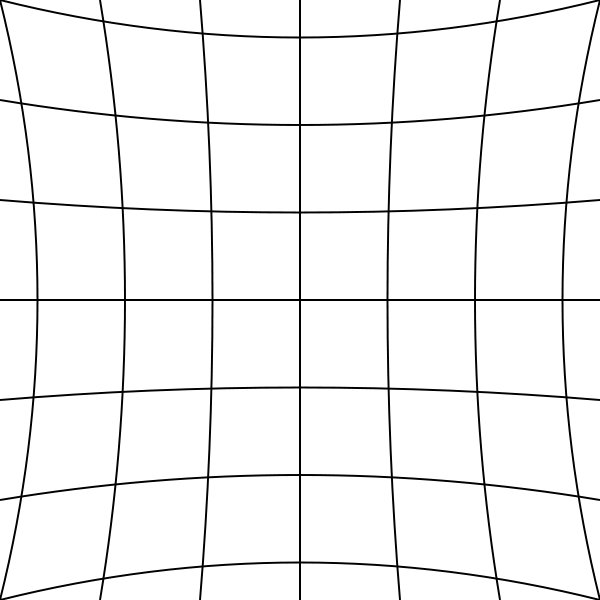
\includegraphics[width=3cm]{img/600px-Pincushion_distortion.png}
		\end{minipage}
		\begin{minipage}{3cm}
			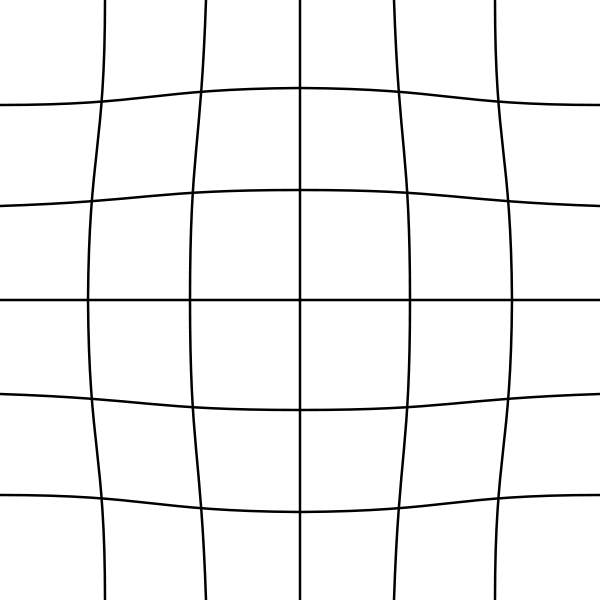
\includegraphics[width=3cm]{img/600px-Mustache_distortion.png}
		\end{minipage}
	\caption{Rodzaje dystorsji}
Kolejno od lewej: beczkowa, poduszkowa oraz falista. \\
Źródło: https://en.wikipedia.org/wiki/Distortion\_\%28optics\%29
	\label{fig:distortion}
\end{figure}

Zaprezentowany wcześniej model zakłada brak zakłóceń przy procesie przetwarzania obrazu. W rzeczywistych kamerach występują różne rodzaje zniekształceń. W dystorsji linie proste z oryginalnej przestrzeni nie są proste na obrazie. Wynika to z fizycznej niedoskonałości układów optycznych. Im dalej od osi optycznej, tym większe zniekształcenie.

W bibliotece OpenCV przewiduje się współczynniki radialne $k_1, ..., k_6$ oraz styczne $p_1$ i $p_2$:
(podawane za dokumentacją OpenCV \cite{Dokumentacja OpenCV})

\begin{gather*}
	x' = \frac{x}{z} \\
	y' = \frac{y}{z} \\
	x'' = x' \frac{1+k_1 r^2 + k_2 r^4 + k_3 r^6}{1+k_4 r^2+k_5 r^4+k_6 r^6} +
	2 p_1 x' y' + p_2(r^2 + 2 x'^2)	\\
	y'' = y' \frac{1+k_1 r^2 + k_2 r^4 + k_3 r^6}{1+k_4 r^2+k_5 r^4+k_6 r^6} +
	p_1(r^2 + 2 y'^2) + 2 p_2 x' y'
\end{gather*}

Współczynniki te następnie są wykorzystywane we wcześniejszym modelu w następujący sposób:

\begin{gather*}
	u = f_x x'' + c_x \\
	v = f_y y'' + c_y
\end{gather*}

Widać, że uzwględnienie współczynników dystorsji znacznie komplikuje przyjęty model, jednakże jest koniecznym krokiem przed przystąpieniem do dalszych operacji.

\subsection{Kalibracja kamery}

Kalibracja kamery odbywa się poprzez fotografowanie czarno-białej szachownicy pod różnymi kątami. Następnie zdjęcia są konwertowane do skali szarości i wykrywane są narożniki szachownicy. Pierwsze oszacowanie położenia narożników nie jest dokładne. Estymacja jest poprawiana z wykorzystaniem prostego faktu dotyczącego gradientu:

\begin{figure}
\centering
	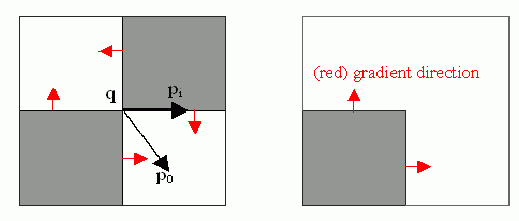
\includegraphics[width=0.70\textwidth]{img/cornersubpix.png}\par\vspace{1cm}
\caption{Gradient szachownicy}
źródło: https://docs.opencv.org/2.4/modules/imgproc/doc/feature\_detection.html
	\label{fig:gradient}
\end{figure}

Załóżmy, że $\bb{q}$ jest narożnikiem szachownicy, a $\bb{p}_i$ jest punktem w bliskim sąsiedztwie. Przyjmijmy, że wartość błędu dana jest następującym równaniem:

\begin{equation}
	E_i = \nabla f_{\bb{p}_i}^T (\bb{q} - \bb{p}_i)
\end{equation}
gdzie $\nabla f_{\bb{p}_i}$ jest gradientem w punkcie $p_i$. Jest to równanie na iloczyn skalarny i będzie ono równe zero, gdy $\bb{p}_i$ będzie prostopadłe do gradientu. Przyrównując powyższe równanie do zera oraz mnożąc obie strony przez $\nabla f_{\bb{p}_i}$, otrzymujemy:

\begin{align*}
	\nabla f_{\bb{p}_i} \nabla f_{\bb{p}_i}^T \bb{q} - \nabla f_{\bb{p}_i} \nabla f_{\bb{p}_i}^T \bb{p}_i = 0
\end{align*}

W konsekwencji otrzymujemy:

\begin{align}
	\bb{q} = (\nabla f_{\bb{p}_i} \nabla f_{\bb{p}_i}^T)^{-1} \nabla f_{\bb{p}_i} \nabla f_{\bb{p}_i}^T \bb{p}_i
\end{align}

Operacja ta jest powtarzana, aż punkt $q$ uzyska stabilną wartość (jego współrzędne nie będą się zmieniać o większą wartość niż przyjęty próg).

\begin{figure}
\centering
		\begin{minipage}{3.5cm}
			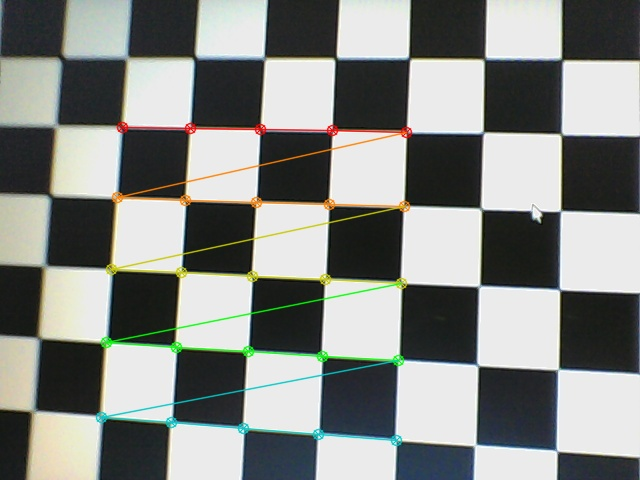
\includegraphics[width=3.5cm]{img/left1.jpg}
		\end{minipage}
		\begin{minipage}{3.5cm}
			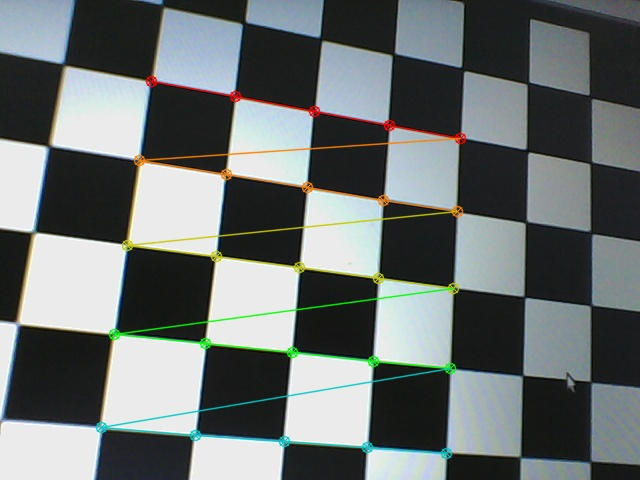
\includegraphics[width=3.5cm]{img/left10.jpg}
		\end{minipage}
		\begin{minipage}{3.5cm}
			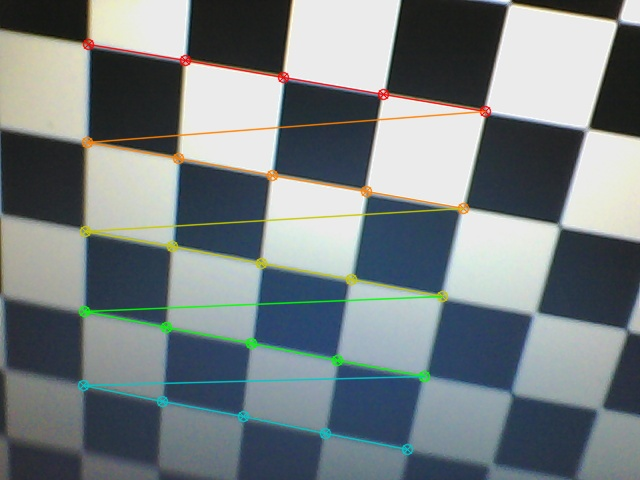
\includegraphics[width=3.5cm]{img/left27.jpg}
		\end{minipage}
	\caption{Wykryte narożniki szachownicy}
	\label{fig:corners}
\end{figure}

\begin{figure}
\centering
		\begin{minipage}{3.5cm}
			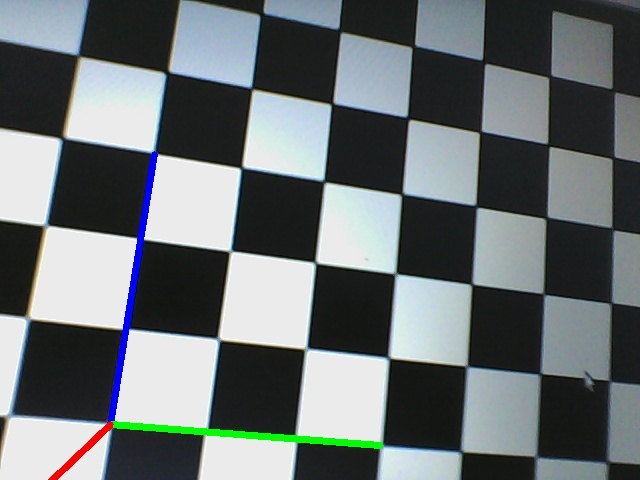
\includegraphics[width=3.5cm]{img/left8.jpg}
		\end{minipage}
		\begin{minipage}{3.5cm}
			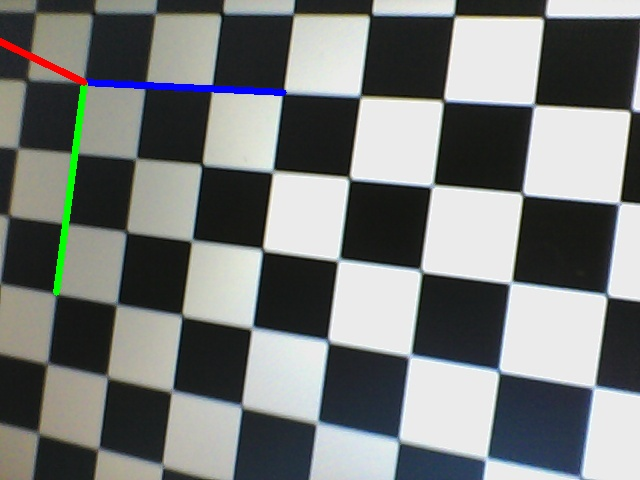
\includegraphics[width=3.5cm]{img/left17.jpg}
		\end{minipage}
		\begin{minipage}{3.5cm}
			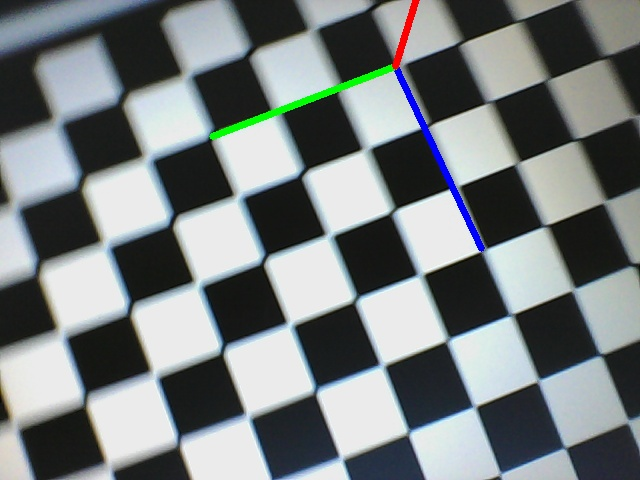
\includegraphics[width=3.5cm]{img/left24.jpg}
		\end{minipage}
	\caption{Estymacja orientacji szachownicy}
	\label{fig:pose}
\end{figure}

Dzięki wyznaczonym narożnikom można określić wewnętrzne i zewnętrzne kamery. Wartości te są następnie wykorzystane do estymacji pozycji (Rys. \ref{fig:pose}) oraz do usunięcia zakłóceń z obrazu. 

\subsection{Geometria epipolarna}

Zakładając wcześniej przyjęty model rzeczywistej kamery oraz stosując uproszczenie, polegające na przeniesieniu płaszczyzny obrazu przed ognisko (w rzeczywistych kamerach płaszczyzna ta znajduje się za ogniskiem), możemy zauważyć pewne zależności geometryczne dla punktu widzianego z dwóch kamer. 

\begin{figure}
\centering
	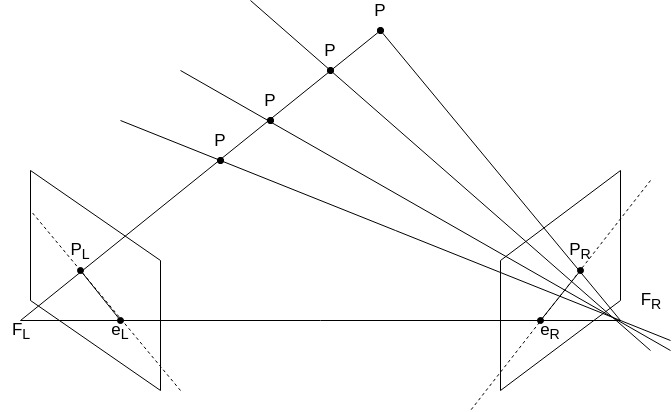
\includegraphics[width=0.70\textwidth]{img/epipolar.jpg}\par\vspace{1cm}
\caption{Podstawowa koncepcja geometrii epipolarnej}
	\label{fig:epipolar_scene}
\end{figure}

Analizując scenę przedstawioną na Rys. \ref{fig:epipolar_scene} można zauważyć, że ogniska obu kamer, punkt P oraz jego projekcje na płaszczyznę obrazu, leżą na jednej płaszczyźnie. Linia poprowadzona między ogniskami kamer jest nazywana linią główną (ang. baseline). 
Punkty przecięcia linii głównej z płaszczyzną główną ($e$), nazywane są epipolami (ang. epipoles). Jeśli obie kamery znajdują się w swoim polu widzenia, to epipole są widoczne jako środek drugiej kamery na obrazie.
Płaszczyzna przechodząca przez dowolny punkt P, widziany w~obu kamerach oraz przez linię główną, jest nazywana płaszczyzną epipolarną.
Linią epipolarną nazywamy linię, znajdującą się na przecięciu płaszczyzny obrazu z płaszczyzną epipolarną. Wszystkie linie epipolarne przecinają się w epipolach.

Warto zwrócić uwagę na to, że linia $F P$ jest widziana na drugim obrazie jako linia epipolarna. Oznacza to więc, że szukając odpowiednika piksela z jednego obrazu na drugim, należy szukać wzdłuż epilinii, a nie na całym obrazie. Jest to istotne ułatwienie, które będzie miało duże znaczenie przy obliczaniu dysparycji.

\subsection{Szacowanie głębokości}

Kolejnym krokiem jest obliczenie mapy dysparycji oraz na jej podstawie wyznaczenie głębokości. 

\begin{figure}
	\centering
	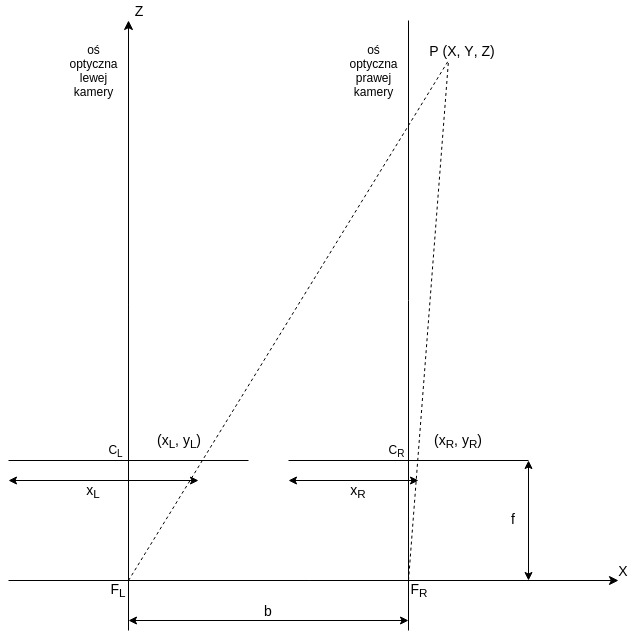
\includegraphics[width=9.5cm]{img/ekstrakcja.jpg}
	\caption{Ekstrakcja głębi na podstawie dysparycji obrazów z dwóch kamer}
	\label{fig:extraction}
\end{figure}

Przy ekstrakcji głęgokości korzysta się z podobieństwa trójkątów $P F_L F_R$ oraz $P C_L C_R$ z Rys. \ref{fig:extraction}:

\begin{equation}
	\frac{b}{Z} = \frac{b-x_L+x_R}{Z-f}
	\label{eq:disp}
\end{equation}

Po przekształceniach otrzymujemy:

\begin{equation}
	Z = \frac{bf}{x_L-x_R} = \frac{bf}{d}
\end{equation}
gdzie $d$ jest dysparycją - różnicą wartości odpowiadających sobie pikseli na dwóch obrazach szukanych wzdłuż epilinii.
Znając ogniskową, odległość między kamerami oraz obliczając różnicę między analogicznymi pikselami z dwóch obrazów możemy szacować głębię.

Warto zwrócić uwagę, że wzór (\ref{eq:disp}) nie traci na ogólności, gdy punkt $P$ znajdzie się pomiędzy osiami optycznymi kamer, ponieważ do obliczenia podstawy trójkąta $P C_L C_R$ zostanie wykorzystana odległość między osią optyczną prawej kamery, a punktem, w którym wiązka światła pada na prawą matrycę. Odległość ta może zostać w takim wypadku wyrażona jako $\frac{1}{2}l-x_R$, gdzie $l$ to długość ekranu światłoczułego. Po podstawieniu podobnej wartości za odległość od osi optycznej lewej kamery do punktu przecięcia wiązki światła z lewą matrycą $\frac{1}{2}l$ uprości się i zostaniemy ze wzorem (\ref{eq:disp}).

\begin{figure}
	\centering
	\begin{minipage}{5.5cm}
		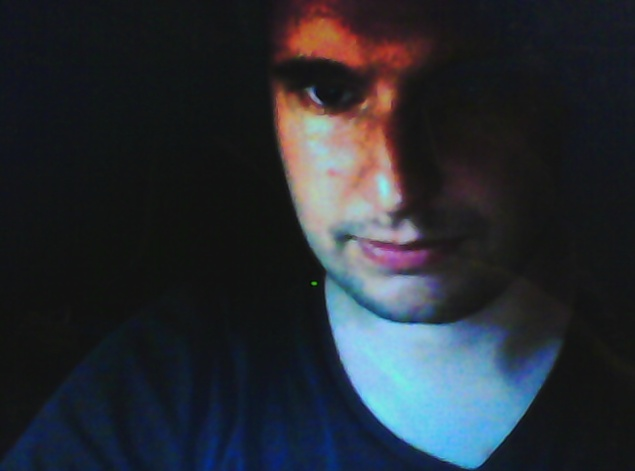
\includegraphics[width=5.5cm]{img/falt_test_face1L.jpg}
	\end{minipage}
	\begin{minipage}{5.5cm}
		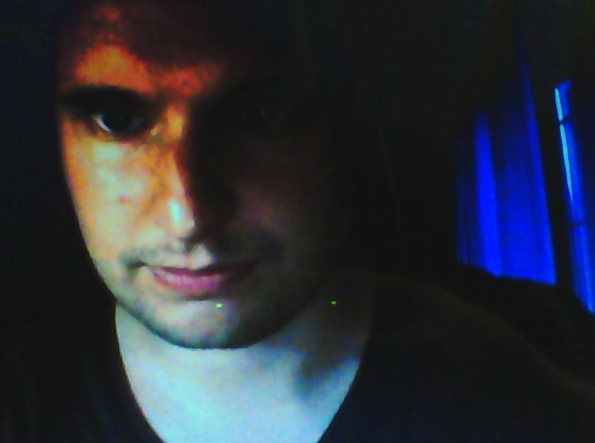
\includegraphics[width=5.5cm]{img/falt_test_face1R.jpg}
	\end{minipage}
	
	\centerline{
	\begin{minipage}{10.5cm}
		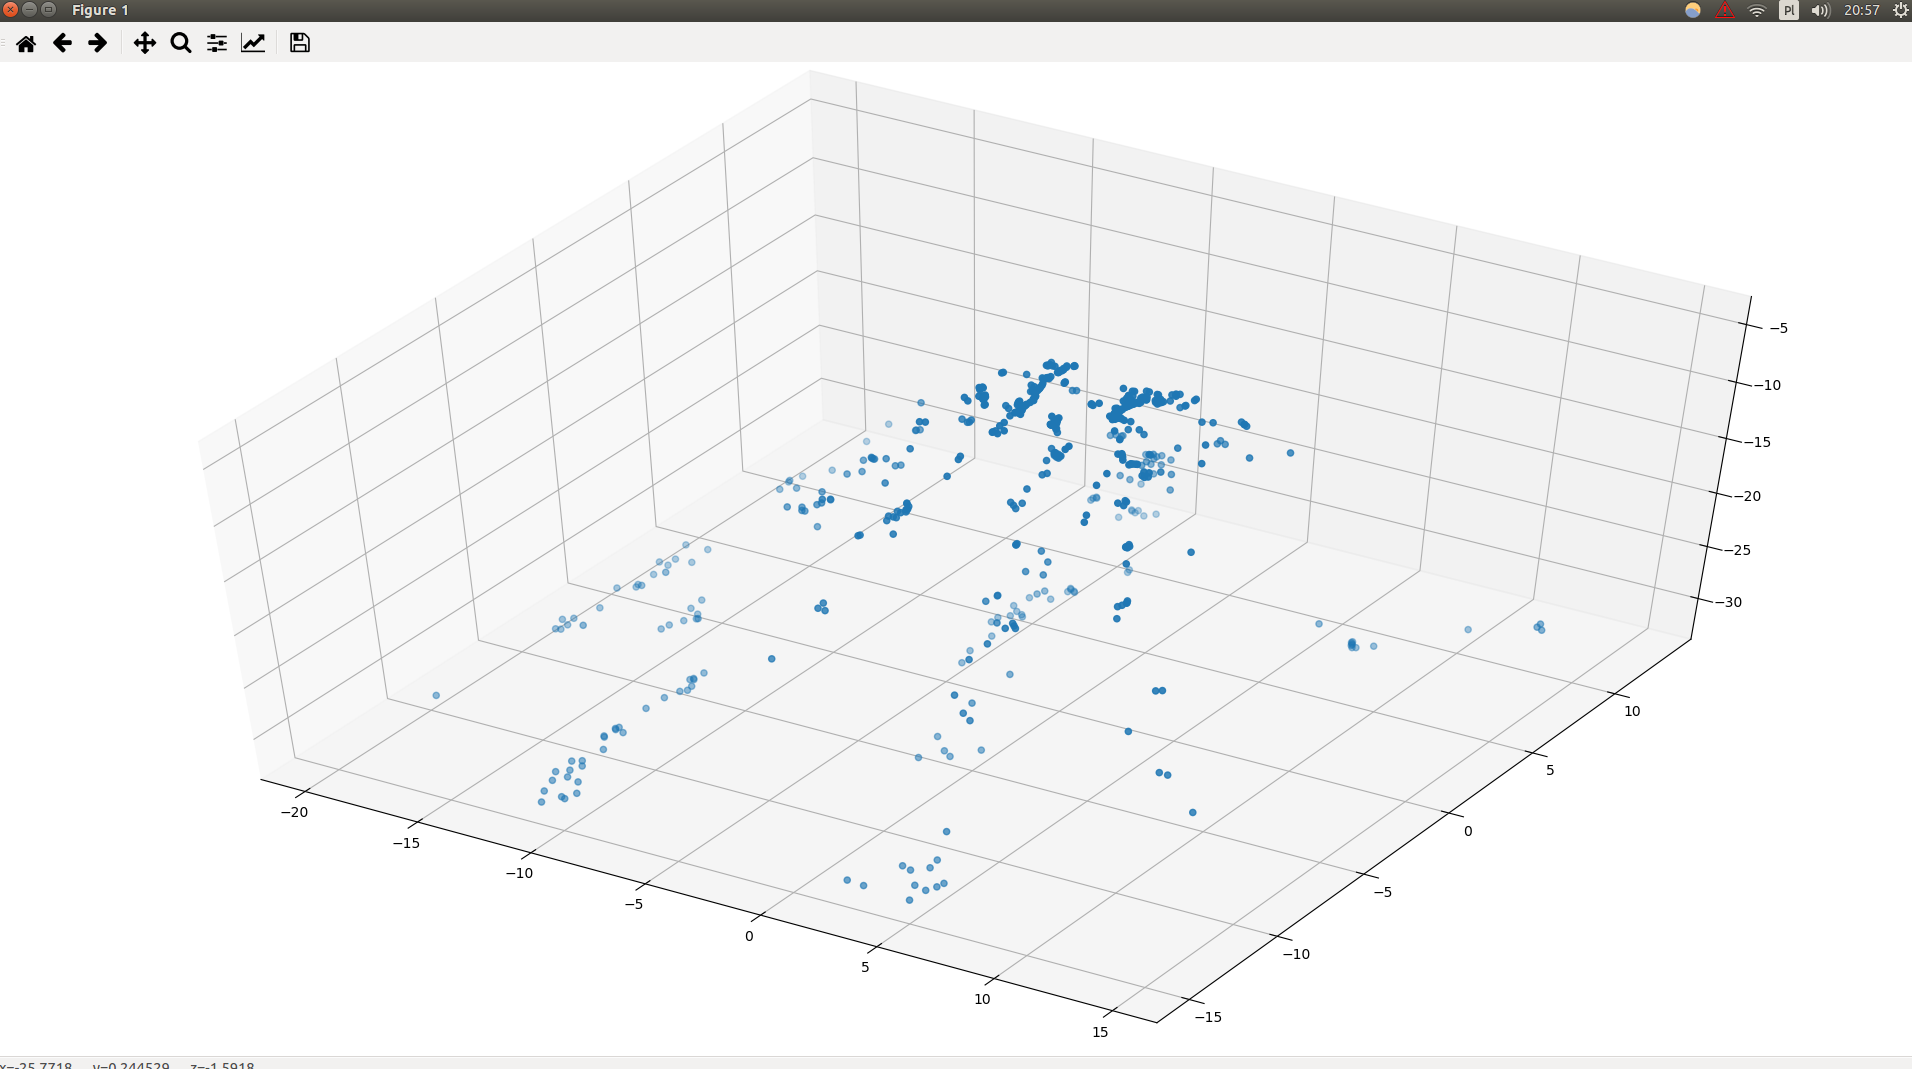
\includegraphics[width=10.5cm]{img/result_fail.png}
	\end{minipage}}	
	\caption{Obraz płaskiego zdjęcia, sfotografowany lewą i prawą kamerą oraz wynik ekstrakcji głebokości}
	\label{fig:extraction_fail}
\end{figure}


\section{Wyniki}
Dokonano kalibracji kamery i wyznaczono jej współczynniki wewnętrzne i zewnętrzne. Jednakże nie udało się uzyskać zadowalających rezultatów. Po przedstawieniu systemowi zdjęcia osoby wyświetlonego na laptopie, uzyskano mapę głębi przedstawioną na Rys. \ref{fig:extraction_fail}. Jak można z łatwością zauważyć, na mapie głębokości otrzymano punkty o różnej wartości współrzędnej z, czyli systemowi nie udało się poprawnie zidentyfikować płaskiej powierzchni. Gdyby uzyskana mapa głębi była z dopuszczalnym błędem aproskymowalna płaszczyną, kolejnym krokiem byłoby zobserwowanie, jak system zachowuje się dla realnej twarzy. Na podstawie obserwacji oraz występujących błędów aproksymacji płaszczyzną, planowano ustalić próg błędu aproksymacji. Po przekroczeniu takiego progu, system mógłby uznać, że podejmowana jest próba oszustwa.

Trudno jest określić jedną przyczynę niepowodzenia. Na pewno ważną rolę odgrywa kalibracja kamer. Wielokrotnie podejmowano próbę poprawiania uzyskiwanych wyników poprzez ponowną kalibrację, ale nie wpłynęło to w znaczący sposób na rezultaty. W~związku z ograniczoną ilością czasu, projekt nie mógł zostać ukończony pomimo wielu godzin poświęconych na analizę problemu.



\chapter{Zakończenie}

\section{Podsumowanie projektu}

W trakcie pracy nad projektem udało się zrealizować następujące zadania:
\begin{itemize}

\item Ustalono protokoły komunikacji z innymi komponentami.

\item Wykorzystano implementację alogrytmu kaskad Haara do wykrycia, czy na zdjęciu jest twarz ludzka oraz do wyznaczenia współrzędnych twarzy.

\item Przeanalizowano działanie algorytmu PCA, pozwalającego na redukcję wymiarowości i wykorzystano go do przygotowania wektora uczącego dla sieci neuronowej.

\item Przetestowano poprawność działania całego systemu.

\item Zaproponowano alternatywne metody rozwiązania postawionego problemu.

\item Zbadano jakie możliwości w projekcie może oferować ekstrakcja głębi na podstawie obrazów z dwóch kamer.

\end{itemize}

Rozwiązanie zaproponowane w projekcie cieszy się dużą popularnością i daje wystarczająco dobre rezultaty. Praca z wykorzystaniem algorytmu PCA jest wygodna, ponieważ dane, którymi operujemy mają geometryczną interpretację. Dodatkowym atutem w analizowanym zastosowaniu PCA, jest możliwość wizualizacji rezultatów, co ułatwia weryfikację otrzymanych wyników. Ze względu na dużą dostępność bibliotek, w trakcie realizacji projektu przywiązano większą wagę do zrozumienia podstaw działania algorytmów. W~pracy starano się unikać bezpośrednich odwołań do sposobu działania bibliotek, raczej skupiano się na fundamentach teoretycznych, analizowanych algorytmów. Owocem takiego podejścia jest prostota zrealizowanego komponentu pod kątem programistycznym, przy jednoczesnym spełnieniu głównego celu postawionego przed rozpoczęciem realizacji projektu: zwiększenie wiedzy na temat stosowanych rozwiązań w dziedzinie Pattern Recognition. 

W projekcie nie przeprowadzono testów modułowych komponentu, system był testowany jako całość. Powodem takiego stanu rzeczy jest trudność w testowaniu omawianego komponentu, ze względu na jego dość abstrakcyjny charakter, w porównanianu do reszty systemu. Testowanie rezultatów działania całego systemu jest czasochłonne. Dowolna zmiana w systemie ekstrakcji cech powoduje konieczność rozpoczynania procesu uczenia sieci neuronowej od nowa. W dalszej części tego rozdziału przedstawiono pomysł na zaimplementowanie testów modułowych dla komponentu realizującego ekstrakcję cech.

Realizowany projekt umożliwił opracowanie i wykorzystanie wydajnych sposobów na pracę w grupie. Komponentowe podejście do systemu umożliwiło prowadzenie równoległych prac nad rozwojem całego systemu. Ustalenie abstrakcyjnych interfejsów między komponentami pozwoliłoby na przeprowadzanie daleko idących zmian w obrębie komponentu, bez konieczności wprowadzania zmian w innych częściach systemu.

\section{Możliwe usprawnienia}

System jako całość w obecnym stanie spełnia podstawowe założenia, jakie zostały przed nim postawione, t.j. rozpoznawanie twarzy niewielkiej grupy osób oraz ich identyfikacja. Jednakże jest wiele aspektów, które można poprawić i rozwinąć. W niniejszej sekcji przeprowadzono dyskusję najważniejszych problemów, które należy zaadresować przy dalszej pracy nad projektem.

\subsubsection{Testy modułowe}

Jednym z pomysłów na rozwój systemu jest porównanie efektów działania algorytmów redukcji wymiarowości. Metodyka takich testów miałaby polegać na utworzeniu bazy zdjęć różnych osób i porównaniu odległości współrzędnych, przyporządkowanych danym zdjęciom z bazy przez różne algorytmy. Możliwe do analizowania miary to: średnia odległość, największa i najmniejsza odległość, mediana oraz wariancja. Przy takim porównaniu należy oczywiście wybrać odpowiedni rodzaj normy. Takie podejście umożliwiłoby uniezależnienie wyników omawianego komponentu od sieci neuronowej, co znacznie ułatwiłoby badania właściwości proponowanych rozwiązań. Warto zwrócić uwagę, że takie rozwiązanie pozwala na testowanie dowolnego podejścia do problemu. Ustalenie wspólnego zbioru zdjęć dla porównywanych algorytmów, normy dla przestrzeni cech oraz miar i progów dla każdej z miar, umożliwiłoby automatyzację testów.


\subsubsection{Zbadanie wpływu czynników wizualnych na wyniki systemu}
Mając dostęp do usystematyzowanych testów można dokładnie zbadać wyniki, jakie osiąga system oraz jego odporność na czynniki wizualne. Do takich czynników zalicza się: różne ustawienie twarzy, jej oświetlenie kierunkowe, pory dnia, zarost czy okulary. Proponuje się przyjęcie zbioru zdjęć jednej osoby w różnych warunkach oświetleniowych i porównanie uzyskanych wektorów.

\subsubsection{Geometryczne cechy}
W rozdziale \ref{geometrical_features} przedstawiono sposób na wykorzystanie innego rodzaju cech. Koncpecja ta polega na przygotowaniu wektora cech z geometryczną interpretacją. Każdy element takiego wektora mógłby oznaczać odległość między charakterystycznymi punktami twarzy. Aby uniezależnić uzyskiwane wyniki od odległości, wszystkie odległości muszą być względne. W przypadku tego typu wektora należy przetestować, jak sieć neuronowa poradzi sobie z tego typu cechami oraz zbadać wpływ pozy twarzy na osiągane wyniki. Algorytmy estymujące położenie punktów charakterystycznych z reguły potrafią sobie poradzić z oświetleniem, więc nie byłby to czynnik mający wielkie znaczenie w tym przypadku, można go jednakże dodać do testów dla podwójnego sprawdzenia.

\subsubsection{Ekstrakcja głębi}
Ekstrakcja głębi na podstawie obrazów z dwóch kamer w obecnym stanie projektu nie daje zadowalających rezultatów. Fakt ten prawdopodobnie jest spowodowany złą kalibracją kamery, niewłaściwym położeniem kamer, bądź niewłaściwym określeniem położenia kamer. Jest to część projektu, która musi zostać dopracowana, następnie może zostać zintegrowana z resztą systemu. Poza zwiększeniem bezpieczeństwa systemu można wykorzystać mapę głębi do ekstrakcji cech. Ponieważ taka mapa ma zbyt wiele punktów, konieczne byłoby wykorzystanie algorytmów redukcji wymiarowości. Bardzo ciekawe mogłoby być porównanie wyników uzyskiwanych przez system na podstawie obrazów 2D i~3D. Informacje uzyskane dzięki estymacji głębi otwierają bardzo wiele możliwości rozwoju systemu.


\newpage
\begin{thebibliography}{9}

\bibitem{Pattern recognition}
Christopher M. Bishop.
\textit{Pattern recognition and machine learning}.
Springer Science + Business Media, New York 2009

\bibitem{Ślot}
Krzysztof Ślot.
\textit{Rozpoznawanie biometryczne. Nowe metody ilościowej reprezentacji obiektów}
Wydawnictwo Komunikacji i Łączności, Warszawa 2000

\bibitem{Osowski}
Stanisław Osowski.
\textit{Sieci Neuronowe w ujęciu algorytmicznym}
Wydawnictwo Naukowo-Techniczne, Warszawa 1996

\bibitem{Wzorce projektowe}
Erich Gamma, Richard Helm, Ralph Johnson, John Vlissides
\textit{Wzorce projektowe. Elementy oprogramowania obiektowego wielokrotnego użytku}
Wydawnictwo Helion, Gliwice 2017

\bibitem{Clean Code}
Martin, Robert C.
\textit{Czysty Kod}
Wydawnictwo Helion, Gliwice 2014


\bibitem{AdaBoost}
Yoav Freund, Robert E. Schapire.
\textit{A Short Introduction to Boosting}
Journal of Japanese Society for Artificial Intelligence, 1999

\bibitem{Kaskada Haara}
Paul Viola, Michael Jones.
\textit{Rapid Object Detection using a Boosted Cascade of Simple Features}.
Cambridge 2001

\bibitem{Landmark face detector}
Vahid Kazemi, Josephine Sullivan.
\textit{One Millisecond Face Alignment with an Ensemble of Regression Trees}
KTH, Royal Institute of Technology
Computer Vision and Active Perception Lab, 2014

\bibitem{NMF}
Daniel D. Lee and Seung, H. Sebastian.
\textit{Advances in Neural Information Processing Systems 13: Algorithms for Non-negative Matrix Factorization}
str. 556-562
MIT Press, 2001

\bibitem{NMF_SVD}
C. Boutsidis, E. Gallopoulos.
\textit{SVD based initialization: A head start for nonnegative matrix factorization}
University of Patras 2007

\bibitem{ICA}
Aapo Hyvärinen, Erkki Oja
\textit{Independent Component Analysis: Algorithms and Applications}
Helsinki University of Technology, 2000

\bibitem{Stereo}
Hartley, R.~I., Zisserman, A.
\textit{Multiple View Geometry in Computer Vision}
Cambridge University Press, 2004

\bibitem{OpenCV}
Itseez.
\textit{Open Source Computer Vision Library}
\\\texttt{https://github.com/itseez/opencv}

\bibitem{Dokumentacja OpenCV}
Dokumentacja biblioteki OpenCv 
\\\texttt{https://docs.opencv.org/2.4/index.html}

\bibitem{Tutoriale OpenCV}
Zbiór tutoriali z OpenCV
\\\texttt{https://docs.opencv.org/3.0-beta/doc/py\_tutorials/py\_tutorials.html}

\bibitem{scikit-learn}
Pedregosa, F. and Varoquaux, G. and Gramfort, A. and Michel, V.
         and Thirion, B. and Grisel, O. and Blondel, M. and Prettenhofer, P.
         and Weiss, R. and Dubourg, V. and Vanderplas, J. and Passos, A. and
         Cournapeau, D. and Brucher, M. and Perrot, M. and Duchesnay, E.
 \textit{Scikit-learn: Machine Learning in {P}ython}
 Journal of Machine Learning Research, volume 12, strony 2825-2830, 2011
 
\bibitem{Olivetti faces}
Informacje na temat zbioru zdjęć twarzy zawartym w bibliotece scikit-learn.
\\\texttt{http://scikit-learn.org/stable/datasets/olivetti\_faces.html}

\bibitem{FaceID hacked}
News o pokonaniu zabezpieczeń systemu FaceID
\\\texttt{http://www.bkav.com/d/top\-news/\-/view\_content/content/103968/face\-id\-beaten\-by\-mask\-not\-an\-effective\-security\-measure}

\end{thebibliography}

\tableofcontents

\listoffigures

\end{document}